\documentclass{article}
\bibliographystyle{livrevrel}

\usepackage{epubtk}
\usepackage{graphicx}
\usepackage{amsmath}
\usepackage{amssymb}
%\usepackage{latexsym}
\usepackage{textcomp}
\usepackage{xspace}

\showlistoftablesfalse 

%LivRev: instead of $^$ we're often use the \super macro for better HTML
\newcommand{\mum}{\textmu\hspace{-0.2pt}m\xspace}
\newcommand{\muHz}{\textmu\hspace{-0.2pt}Hz\xspace}
\newcommand{\muN}{\textmu\hspace{-0.2pt}N\xspace}
\newcommand{\Hz}{Hz\super{-1/2}\xspace}
\newcommand{\HzHz}{Hz~Hz\super{-1/2}\xspace}

%\newcommand{\miranda}[1]{\textcolor{red}{{\bf Editor, MD: #1}}}  

%livRev: add \enlargethispage{\baselineskip} to \tableofcontents after PREPROCESS

%=========================================================================

\begin{document}

\title{Gravitational Wave Detection by Interferometry \\(Ground and Space)}

\author{%
\epubtkAuthorData{Matthew Pitkin}
        {Scottish Universities Physics Alliance (SUPA)\\
        School of Physics and Astronomy,\
        University of Glasgow \\
        Glasgow G12 8QQ, U.K.}
        {matthew.pitkin@glasgow.ac.uk}
        {}
\and
\epubtkAuthorData{Stuart Reid}
        {Scottish Universities Physics Alliance (SUPA)\\
        School of Physics and Astronomy,
        University of Glasgow \\
        Glasgow G12 8QQ, U.K.}
        {stuart.reid.2@glasgow.ac.uk}
    {}
\and
\epubtkAuthorData{Sheila Rowan}
        {Scottish Universities Physics Alliance (SUPA)\\
        School of Physics and Astronomy,
        University of Glasgow \\
        Glasgow G12 8QQ, U.K.}
        {sheila.rowan@glasgow.ac.uk}
        {}
\and
\epubtkAuthorData{Jim Hough}
        {Scottish Universities Physics Alliance (SUPA)\\
        School of Physics and Astronomy,
        University of Glasgow \\
        Glasgow G12 8QQ, U.K.}
        {james.hough@glasgow.ac.uk}
        {}
}

\date{}
\maketitle


\begin{abstract}
Significant progress has been made in recent years on the development of
gravitational-wave detectors, culminating in the first direct detection of
a gravitational wave signal in September 2015. Sources such as coalescing compact binary
systems, neutron stars in low-mass X-ray binaries, stellar collapses and
pulsars are all possible candidates for detection. A now proven design
of gravitational-wave detector uses test masses a long distance apart and
freely suspended as pendulums on Earth or in drag-free spacecraft.  The
main theme of this review is a discussion of the mechanical and optical
principles used in the various long baseline systems in operation around the
world -- LIGO (USA), Virgo (Italy/France), TAMA300 and KAGRA (Japan), and
GEO600 (Germany/U.K.) -- and in LISA, a proposed space-borne interferometer. A
review of recent science runs from the current generation of ground-based
detectors will be discussed, in addition to highlighting the astrophysical
results gained thus far. Looking to the future, the major upgrades to LIGO
(Advanced LIGO), Virgo (Advanced Virgo), KAGRA and GEO600 (GEO-HF) will be
completed over the coming years, which will create a network of detectors
with the significantly improved sensitivity required to detect
gravitational waves. Beyond this, the concept and design of possible
future ``third generation'' gravitational-wave detectors, such as the
Einstein Telescope (ET), will be discussed.
  
  
\end{abstract}

\epubtkKeywords{gravitational waves, laser interferometry, gravitational wave
detectors, science runs, Interferometric gravitational wave detectors, Noise
sources, Data analysis}

%\newpage

%\epubtkUpdate
%    [Id=A,
%     ApprovedBy=subjecteditor,
%     AcceptDate={17 June 2011},
%     PublishDate={11 July 2011},
%     Type=major]{%
%For the update the author list has changed to be Matthew Pitkin,
%Stuart Reid, Sheila Rowan and Jim Hough. There have been minor updates
%to Sections \ref{section:introduction}, \ref{section:gravwaves} and
%\ref{section:Detection}; major updates to Sections~\ref{section:noise}
%and \ref{section:interferometry}; Section~\ref{section:construction}
%has been renamed and includes entirely new material on the operation
%of, and results from, the first generation of gravitational wave
%detectors and upgrades that are under way; and
%Section~\ref{section:space} also includes major updates about the
%status of LISA. The number of references has increased from 110 to 324.}


%%%%%%%%%%%%%%%%%%%%%%%%%%%%%%%%%%%%%%%%%%%%%%%%%%%%%%%%%%%%%%%%%%%%%%%%%%%%%%%%
%%%%%%%%%%%%%%%%%%%%%%%%%%%%%%%%%%%%%%%%%%%%%%%%%%%%%%%%%%%%%%%%%%%%%%%%%%%%%%%%
%%%%%%%%%%%%%%%%%%%%%%%%%%%%%%%%%%%%%%%%%%%%%%%%%%%%%%%%%%%%%%%%%%%%%%%%%%%%%%%%

\newpage

\section{Introduction}
\label{section:introduction} 

%Gravitational waves, one of the more exotic predictions of Einstein's General
%Theory of Relativity have, after decades of controversy over their existence,
%finally been detected \cite{GW150914}.

On 14 September 2015, after many decades of searching, the LIGO gravitational wave
observatories made the first direct detection of gravitational waves \cite{GW150914}.
The observed signal was inferred to be produced by the final inspiral and coalescence
of two black holes each of roughly 30 solar masses at a distance of more than one billion
light years. Following the initial detection a second confirmed signal, again from a pair
of black holes, has been observed \cite{GW151226}. These observations have opened up the start of
gravitational waves astronomy, with sources such as coalescing neutron star binary
systems, stellar collapses and pulsars all being possible candidates for future detections.
Such observations will significantly boost our understanding of the
Universe. New unexpected sources will almost certainly be found and time will
tell what new information such discoveries will bring.

Gravitational waves, a direct predictions of Einstein's General
Theory of Relativity, are ripples in the curvature of space-time and manifest themselves as fluctuating
tidal forces on masses in the path of the wave. The first gravitational-wave
detectors were based on the effect of these forces on the fundamental resonant
mode of aluminium bars at room temperature. Initial instruments were constructed
by Joseph Weber~\cite{Weber1, Weber2} and subsequently developed by others.
Reviews of this early work are given in~\cite{Tyson, Douglass}. Following the
lack of confirmed detection of signals, aluminium bar systems operated at and
below the temperature of liquid helium were developed~\cite{Astone, Prodi,
Amaldi, Heng}, although work in this area is now subsiding. Until recently the two
detectors, Auriga~\cite{AURIGA} and Nautilus~\cite{NAUTILUS} continued to
operate in an ``astrowatch'' mode, although were shut down in October 2016. A good review of the running of these resonant bar detectors can be found in~\cite{Pizzella2016}. Effort also continues to be pursued into cryogenic spherical bar
detectors, which are designed to have a wider bandwidth than the cylindrical
bars, with the prototype Brazilian detector M\'{a}rio Schenberg~\cite{Schenberg, Aguiar:2006} still under active development (work on the
Dutch MiniGRAIL~\cite{MiniGRAIL, Gottardi:2007} detector is no longer proceeding).
However, the most promising design of gravitational-wave detectors, offering the
possibility of very high sensitivities over a wide range of frequency, uses
widely-separated test masses freely suspended as pendulums on Earth or
in a drag-free craft in space; laser interferometry provides a means
of sensing the motion of the masses produced as they interact with a
gravitational wave.


Ground-based detectors of this type, based on the pioneering work of Forward
and colleagues (Hughes Aircraft)~\cite{Forward}, Weiss and colleagues (MIT)
\cite{Weiss}, Drever and colleagues (Glasgow/Caltech) \cite{Drever1,
Drever2} and Billing and colleagues (MPQ Garching)~\cite{Billing}, will be
used to observe sources whose radiation is emitted at frequencies above a few
Hz, and space-borne detectors, as originally envisaged by Peter Bender and Jim
Faller~\cite{BenderFaller1, BenderFaller2} at JILA, will be developed for
implementation at lower frequencies.


Gravitational-wave detectors of long baseline have been built in a number of
places around the world; in the USA (LIGO project led by a Caltech/MIT
consortium)~\cite{LIGOS5, LIGOweb}, in Italy (Virgo project, a joint
Italian/French venture)~\cite{Acernese:2007, VIRGOweb}, in Germany (GEO600
project built by a collaboration centred on the University of Glasgow, the
University of Hannover, the Max Planck Institute for Quantum Optics, the Max
Planck Institute for Gravitational Physics (Albert Einstein Institute), Golm and
Cardiff University)~\cite{Willke:2007, GEOweb} and in Japan (TAMA300
project)~\cite{TAMAStatus, TAMAweb}. A space-borne detector, called
LISA~\cite{LISA, NASAweb, ESAweb}, was until earlier this year (2011)
under study as a joint ESA/NASA mission as one L-class candidate
within the ESA Cosmic Visions program (a recent meeting detailing
these missions can be found here~\cite{ESACosmicVisions}). Funding
constraints within the US now mean that ESA must examine the
possibility of flying an L-class mission with European-only
funding. The official ESA statement on the next steps for LISA can be
found here~\cite{LISAESAstatement}. When completed, this detector
array would have the capability of detecting gravitational wave
signals from violent astrophysical events in the Universe, providing
unique information on testing aspects of general relativity and
opening up a new field of astronomy.


It is also possible to observe the tidal effects of a passing gravitational
wave by Doppler tracking of separated objects. For example, Doppler tracking of
spacecraft allows the Earth and an interplanetary spacecraft to be used as test
masses, where their relative positions can be monitored by comparing the nearly
monochromatic microwave signal sent from a ground station with the coherently
returned signal sent from the spacecraft~\cite{Estabrook:1975}. By comparing
these signals, a Doppler frequency time series $\Delta \nu / \nu_0$, where
$\nu_0$ is the central frequency from the ground station, can be generated.
Peculiar characteristics within the Doppler time series, caused by the passing
of gravitational waves, can be studied in the approximate frequency band of
10\super{-5} to 0.1~Hz. Several attempts have been made in recent decades to
collect such data (Ulysses, Mars Observer, Galileo, Mars Global Surveyor,
Cassini) with broadband frequency sensitivities reaching 10\super{-16}
(see~\cite{Armstrong:2006} for a thorough review of gravitational-wave
searches using Doppler tracking). There are currently no plans for
dedicated experiments using this technique; however, incorporating
Doppler tracking into another planetary mission would provide a
complimentary precursor mission before dedicated experiments such as
LISA are launched.


The technique of Doppler tracking to search for gravitational-wave signals can
also be performed using pulsar-timing experiments.  Millisecond
pulsars~\cite{Lorimer:2008} are known to be very precise clocks, which
allows the effects of a passing gravitational wave to be observed
through the modulation in the time of arrival of pulses from the
pulsar. Many noise sources exist and, for this reason, it is necessary
to monitor a large array of pulsars over a long observation time.
Further details on the techniques used and upper limits that have been
set with pulsar timing experiments can be found from groups such as
the European Pulsar Timing Array~\cite{Janssen:2008}, the North
American Nanohertz Observatory for Gravitational
Waves~\cite{Jenet:2006,Jenet:2009}, and the Parkes Pulsar Timing
Array~\cite{Hobbs:2008}.


All the above detection methods cover over 13 orders of magnitude in frequency
(see Figure~\ref{fig:fullspectrum}) equivalent to covering from radio waves to
X-rays in the electromagnetic spectrum.  This broadband coverage allows us to
probe a wide range of potential sources.

We recommend a number of excellent books for reference. For a popular account of
the development of the gravitational-wave field the reader should consult
Chapter~10 of \textit{Black Holes and Time Warps} by Kip S.\ Thorne~\cite{Thorne}, or
the more recent books, \textit{Einstein's Unfinished Symphony}, by Marcia
Bartusiak~\cite{Bartusiak:2000} and \textit{Gravity from the Ground Up}, by Bernard
Schutz~\cite{Schutz:2003}. A comprehensive review of developments toward laser
interferometer detectors is found in \textit{Fundamentals of Interferometric
Gravitational Wave Detectors} by Peter Saulson~\cite{Saulsonbook}, and
discussions relevant to the technology of both bar and interferometric detectors
are found in \textit{The Detection of Gravitational Waves} edited by David
Blair~\cite{Blair}.


In addition to the wealth of articles that can be found on the home site of
this journal, there are also various informative websites that can easily be
found, including the homepages of the various international collaborative
projects searching for gravitational waves, such as the LIGO Scientific
Collaboration~\cite{LSCweb}.


  
  


\epubtkImage{figures/full_gw_spectrum/full_gw_spectrum.png}{%
\begin{figure}[htbp]
  \centerline{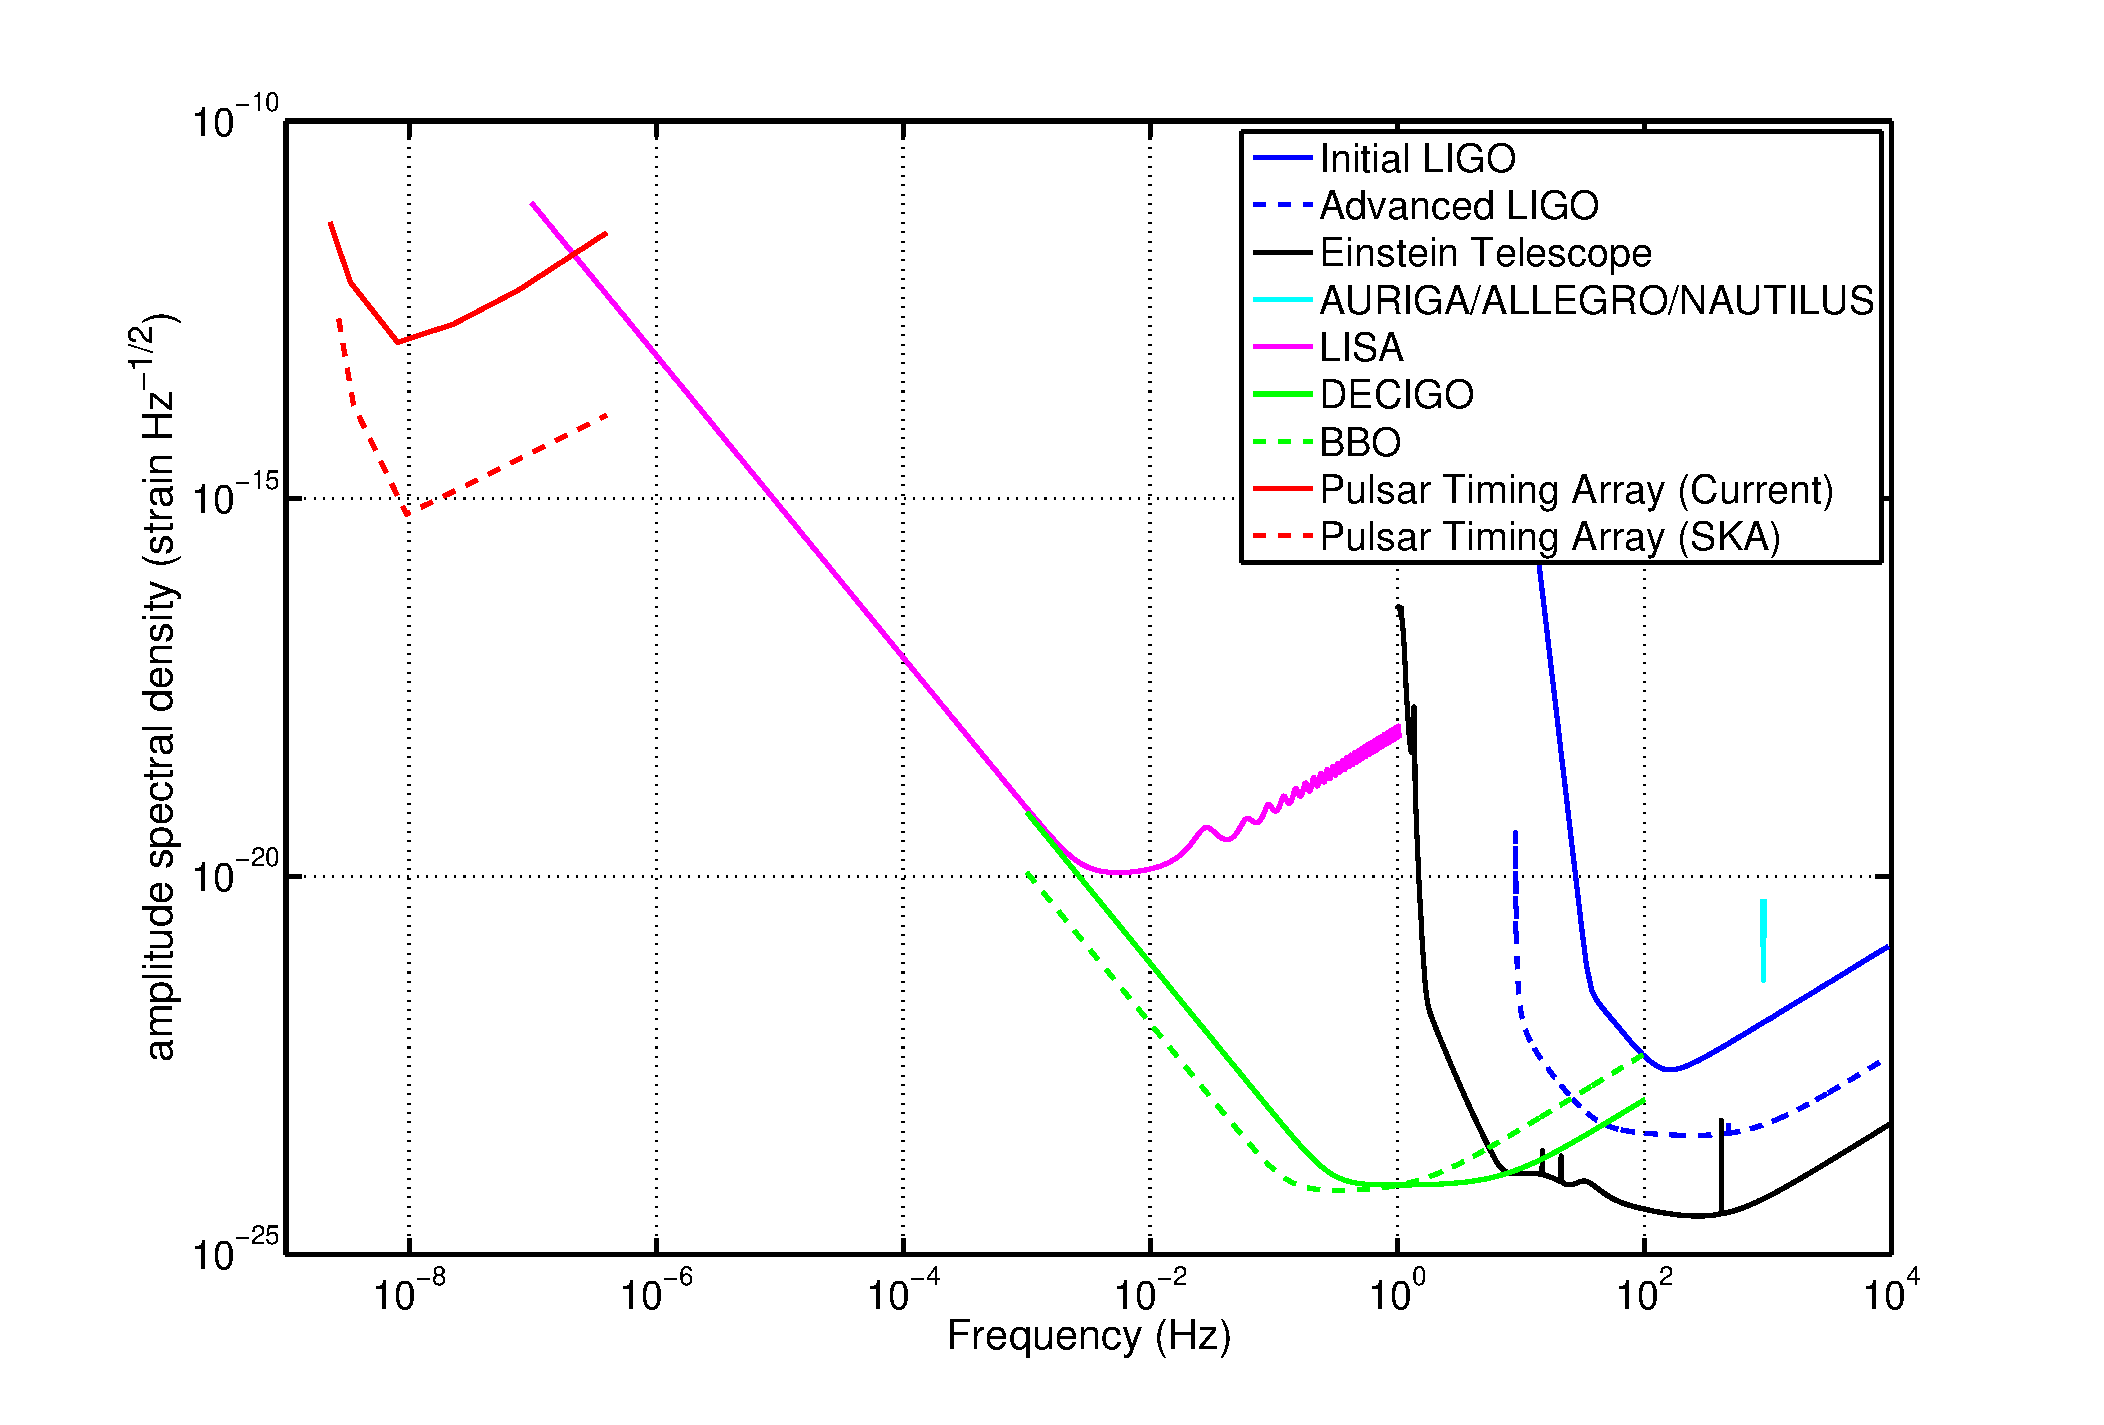
\includegraphics[width=\textwidth]{figures/full_gw_spectrum/full_gw_spectrum}}
  % see http://www.latex-community.org/forum/viewtopic.php?f=5&t=12497 for why the [] is needed
  \caption[]{The sensitivity of various gravitational-wave detection
    techniques across 13 orders of magnitude in frequency. At the low
    frequency end the sensitivity curves for pulsar timing arrays
    (based on current observations and future observations with the
    Square Kilometre Array~\cite{SKA}) are extrapolated from Figure~4
    in~\cite{Yardley:2010}. In the mid-range LISA, DECIGO and BBO are
    described in more detail in Section~\ref{section:space}, with the
    DECIGO and BBO sensitivity curves taken from models given in
    \cite{Yagi:2011}. At the high frequency the sensitivities are
    represented by three generations of laser interferometers: LIGO,
    Advanced LIGO and the Einstein Telescope (see
    Sections~\ref{section:construction}, \ref{subsection:aligo} and
    \ref{subsec:et}). Also included is a representative sensitivity
    for the AURIGA~\cite{AURIGA}, Allegro~\cite{Mauceli:1996} and
    Nautilus~\cite{NAUTILUS} bar detectors.}
\end{figure}}

\newpage

%%%%%%%%%%%%%%%%%%%%%%%%%%%%%%%%%%%%%%%%%%%%%%%%%%%%%%%%%%%%%%%%%%%%%%%%%%%%%%%%
%%%%%%%%%%%%%%%%%%%%%%%%%%%%%%%%%%%%%%%%%%%%%%%%%%%%%%%%%%%%%%%%%%%%%%%%%%%%%%%%

\section{Gravitational Waves}
\label{section:gravwaves} 

Some early relativists were sceptical about the existence of gravitational
waves; however, the 1993 Nobel Prize in Physics was awarded to Hulse and Taylor
for their experimental observations and subsequent interpretations of the
evolution of the orbit of the binary pulsar \epubtkSIMBAD{PSR~1913+16}~\cite{Hulse, Taylor},
the decay of the binary orbit being consistent with angular momentum and energy
being carried away from this system by gravitational waves~\cite{Will}.


Gravitational waves are produced when matter is accelerated in an asymmetrical
way; but due to the nature of the gravitational interaction, detectable levels
of radiation are produced only when very large masses are accelerated in very
strong gravitational fields. Such a situation cannot be found on Earth but is
found in a variety of astrophysical systems. Gravitational wave signals are
expected over a wide range of frequencies; from $\simeq$~10\super{-17}~Hz in the case
of ripples in the cosmological background to $\simeq$~10\super{3}~Hz from the formation
of neutron stars in supernova explosions. The most predictable sources are
binary star systems. However, there are many sources of much-greater
astrophysical interest associated with black-hole interactions and coalescences,
neutron-star coalescences, neutron stars in low-mass X-ray binaries such as
\epubtkSIMBAD[V818~Sco]{Sco-X1}, stellar collapses to neutron stars and black holes (supernova
explosions), pulsars, and the physics of the early Universe. For a full
discussion of sources refer to the material contained in~\cite{Sathyaprakash:2009,LISAsymposium, sources, Amaldiproc}.


Why is there currently such interest worldwide in the detection of gravitational
waves? Partly because observation of the velocity and polarisation states of the
signals will allow a direct experimental check of the wave predictions of
general relativity; but, more importantly, because the detection of the signals
should provide observers with new and unique information about astrophysical
processes. It is interesting to note that the gravitational wave signal from a
coalescing compact binary star system has a relatively simple form and the
distance to the source can be obtained from a combination of its signal strength
and its evolution in time. If the redshift at that distance is found, Hubble's
Constant -- the value for which has been a source of lively debate for many
years -- may then be determined with, potentially, a high degree of
accuracy~\cite{Schutz,Holtz:2005}.


Only now are detectors being built with the technology required to achieve the
sensitivity to observe such interesting sources.


\newpage

\newpage

%%%%%%%%%%%%%%%%%%%%%%%%%%%%%%%%%%%%%%%%%%%%%%%%%%%%%%%%%%%%%%%%%%%%%%%%%%%%%%%%
%%%%%%%%%%%%%%%%%%%%%%%%%%%%%%%%%%%%%%%%%%%%%%%%%%%%%%%%%%%%%%%%%%%%%%%%%%%%%%%%

\section{Detection of Gravitational Waves}
\label{section:Detection} 

Gravitational waves are most simply thought of as ripples in the curvature of
space-time, their effect being to change the separation of adjacent masses on
Earth or in space; this tidal effect is the basis of all present detectors.
Gravitational wave strengths are characterised by the gravitational-wave
amplitude $h$, given by
\begin{equation}
  h = \frac{2 \Delta L} L,
  \label{equation:h}
\end{equation}
where $\Delta L$ is the change in separation of two masses a distance $L$ apart;
for the strongest-allowed component of gravitational radiation, the value of $h$
is proportional to the third time derivative of the quadrupole moment of the
source of the radiation and inversely proportional to the distance to the
source. The radiation field itself is quadrupole in nature and this shows up in
the pattern of the interaction of the waves with matter.


The problem for the experimental physicist is that the predicted magnitudes of
the amplitudes or strains in space in the vicinity of the Earth caused by
gravitational waves even from the most violent astrophysical events are
extremely small, of the order of 10\super{-21} or lower~\cite{Sathyaprakash:2009,
LISAsymposium}. Indeed, current theoretical models on the event rate and strength
of such events suggest that in order to detect a few events per year -- from
coalescing neutron-star binary systems, for example, an amplitude sensitivity
close to 10\super{-22} over timescales as short as a millisecond is required. If
the Fourier transform of a likely signal is considered it is found that the
energy of the signal is distributed over a frequency range or bandwidth, which is
approximately equal to 1/timescale.  For timescales of a millisecond the
bandwidth is approximately 1000~Hz, and in this case the spectral density of the
amplitude sensitivity is obtained by dividing 10\super{-22} by the square root of
1000. Thus, detector noise levels must have an amplitude spectral density lower
than $\simeq$~10\super{-23}~\Hz over the frequency range of the signal.
Signal strengths at the Earth, integrated over appropriate time intervals, for a
number of sources are shown in Figure~\ref{figure:sourcestrengths}.

  

\epubtkImage{figures/fig1/fig1.png}{%
\begin{figure}[htbp]
  \centerline{
\includegraphics[width=0.8\textwidth]{figures/fig1/fig1}}
  \caption[]{\label{fig:fullspectrum}
The sensitivities (given as amplitude spectral densities) of various current and future gravitational-wave detectors
    across $\sim14$ orders of magnitude in frequency. At the low
    frequency end there are estimated sensitivity curves for the current International Pulsar Timing Array and future observations with the
    Square Kilometre Array~\cite{SKA}. In the mid-range are the future space-based detectors LISA, DECIGO and BBO, which are
    described in more detail in Section~\ref{section:space}. At the high frequency the sensitivities are
    represented by three generations of laser interferometers: initial LIGO,
    Advanced LIGO and the Einstein Telescope (see
    Sections~\ref{section:construction}, \ref{subsection:aligo} and
    \ref{subsec:et}). Also shown are a range of potential sources for the detectors, including the gravitational wave signal from GW150914 \cite{GW150914}. This image was created using the GWplotter tool \cite{GWplotter} and a full description of the detector curves used and sources esimates can be found in \cite{2015CQGra..32a5014M}.
  
}
\end{figure}}



The weakness of the signal means that limiting noise sources like the thermal
motion of molecules in the critical components of the detector (thermal noise),
seismic or other mechanical disturbances, and noise associated with the detector
readout, whether electronic or optical, must be reduced to an extremely low
level. For signals above $\simeq$~10~Hz ground based experiments are possible,
but for lower frequencies where local fluctuating gravitational gradients and
seismic noise on Earth become a problem, it is best to consider developing
detectors for operation in space~\cite{LISA}.


\subsection{Initial detectors and their development}
\label{subsection:initdet} 

The earliest experiments in the field were ground based and were carried out by
Joseph Weber of the University of Maryland in the 1960s. With colleagues he
began by looking for evidence of excitation of the normal modes of the Earth by
very low frequency gravitational waves~\cite{Forward2}. Efforts to detect gravitational
waves via the excitation of Earth's normal modes was also pursued by Weiss and Block~\cite{Weiss:1965}.
Weber then moved on to look for tidal strains in aluminium bars, which were at room temperature and were
well isolated from ground vibrations and acoustic noise in the
laboratory~\cite{Weber1, Weber2}. The bars were resonant at $\simeq$~1600~Hz, a
frequency where the energy spectrum of the signals from collapsing stars was
predicted to peak. Despite the fact that Weber observed coincident excitations
of his detectors placed up to 1000~km apart, at a rate of approximately one
event per day, his results were not substantiated by similar experiments carried
out in several other laboratories in the USA, Germany, Britain and Russia. It
seems unlikely that Weber was observing gravitational-wave signals because,
although his detectors were very sensitive, being able to detect strains of the
order of 10\super{-16} over millisecond timescales~\cite{Weber1}, their sensitivity
was far away from what was predicted to be required theoretically. Development
of Weber bar type detectors continued with significant emphasis on cooling to
reduce the noise levels, although work in this area is now subsiding with
efforts continuing on Auriga~\cite{AURIGA}, Nautilus~\cite{NAUTILUS},
MiniGRAIL~\cite{MiniGRAIL, Gottardi:2007} and M\'{a}rio Schenberg
\cite{Schenberg, Aguiar:2006}.  In around 2003, the sensitivity of km-scale
interferometric gravitational-wave detectors began to surpass the peak
sensitivity of these cryogenic bar detectors ($\simeq$~10\super{-21})
and, for example, the LIGO detectors reached their design sensitivities at
almost all frequencies by 2005 (peak sensitivity
$\simeq$~2~\texttimes~10\super{-23} at
$\simeq$~200~Hz)~\cite{Whitcomb:2008}, see
Section~\ref{subsection:runs} for more information on science runs of
the recent generation of detectors.  In addition to gaining better
strain sensitivities, interferometric detectors have a marked
advantage over resonant bars by being sensitive to a broader range of
frequencies, whereas resonant bar are inherently sensitive only to
signals that have significant spectral energy in a narrow band around
their resonant frequency. The concept and design of gravitational-wave
detectors based on laser interferometers will be introduced in the
following Section~\ref{subsection:earth}. 


\subsection{Long baseline detectors on Earth}
\label{subsection:earth} 

An interferometric design of gravitational-wave detector offers the possibility
of very high sensitivities over a wide range of frequency. It uses test masses,
which are widely separated and freely suspended as pendulums to isolate against
seismic noise and reduce the effects of thermal noise; laser interferometry
provides a means of sensing the motion of these masses produced as they interact
with a gravitational wave (Figure~\ref{figure:schematicdetector}).


\epubtkImage{figures/fig2/fig2.png}{%
\begin{figure}[htbp]
  \centerline{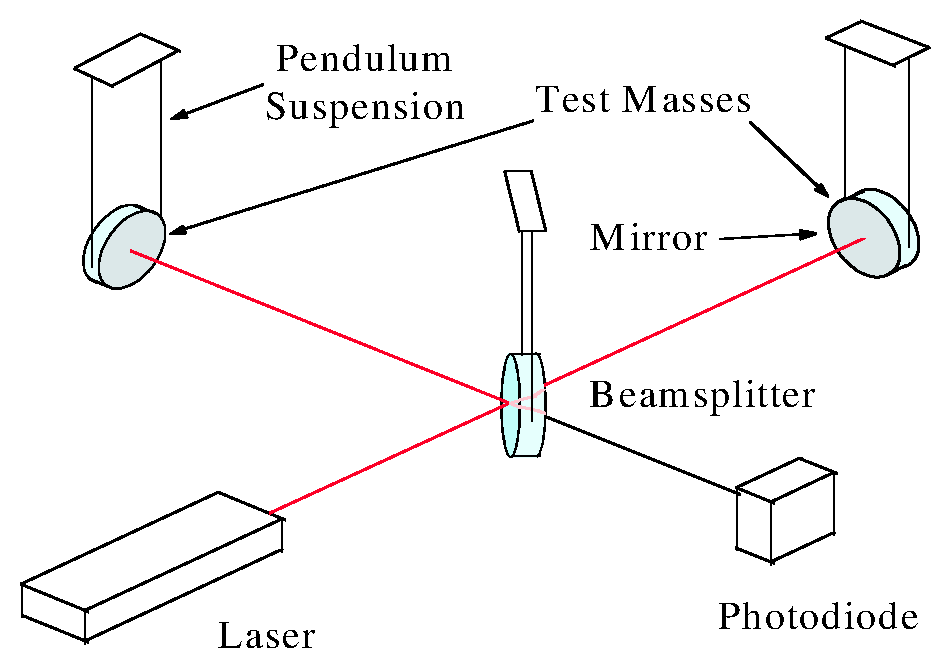
\includegraphics[width=0.5\textwidth]{figures/fig2/fig2}}
  \caption[]{\label{figure:schematicdetector}
Schematic of gravitational-wave detector using laser
    interferometry.}
\end{figure}}

\input{Section3_3}

\epubtkImage{figures/LIGOsens/LIGOsens.png}{%
\begin{figure}[htbp]
  \centerline{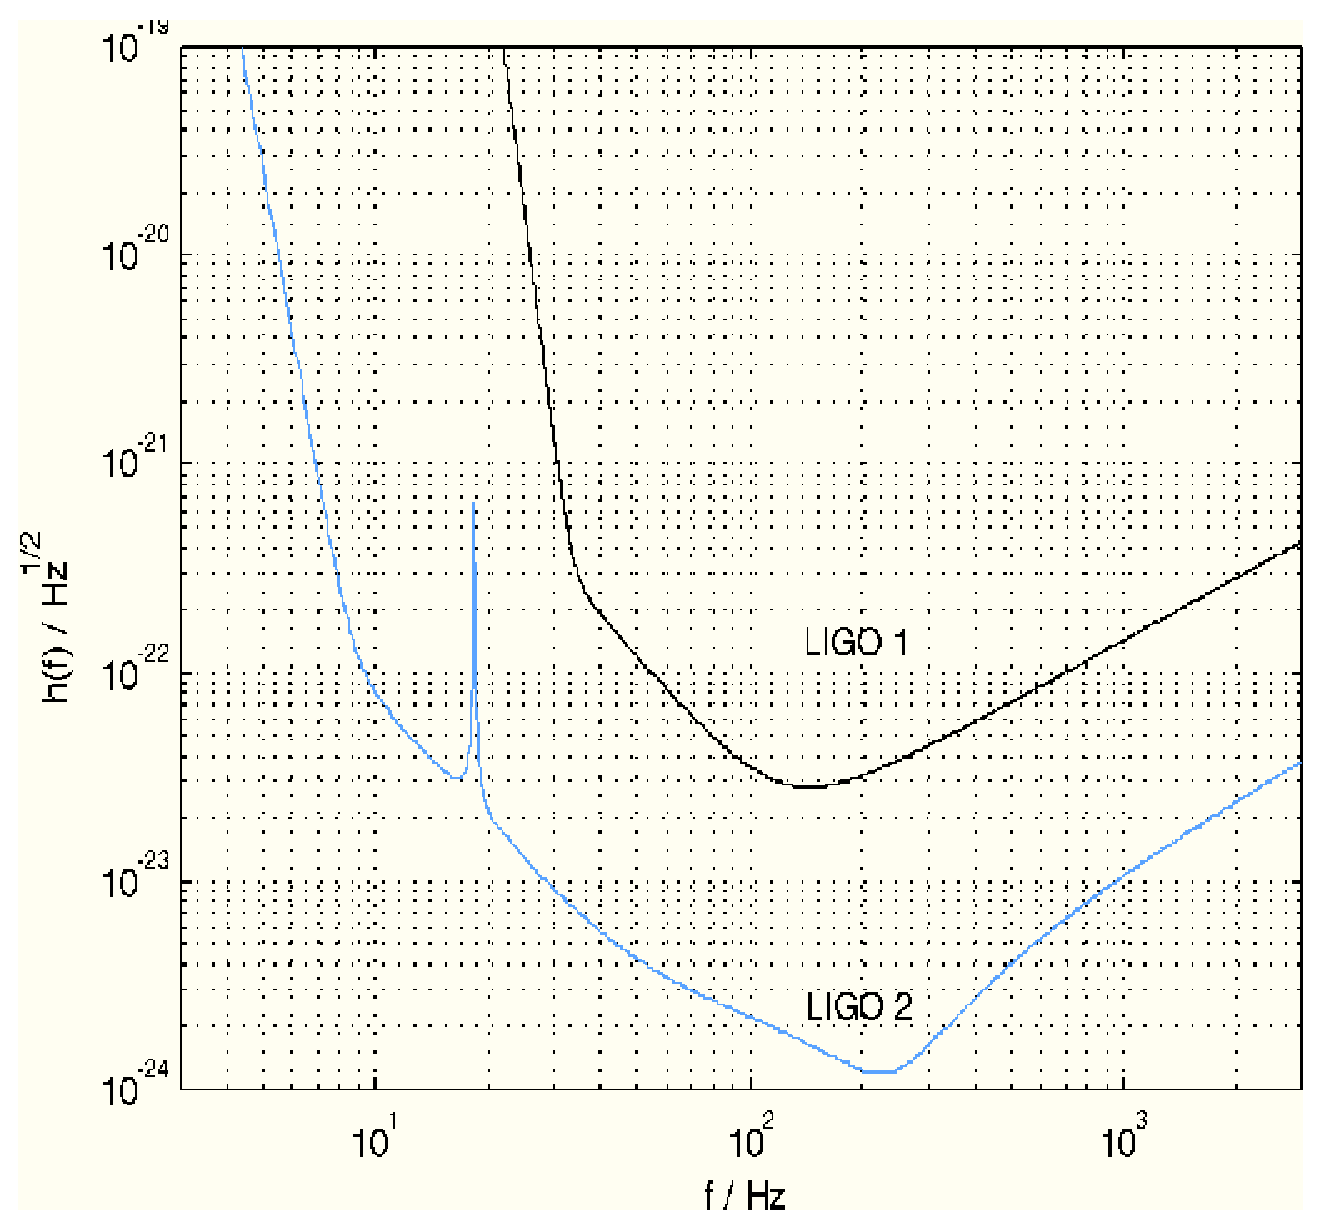
\includegraphics[width=0.9\textwidth]{figures/LIGOsens/LIGOsens}}
  \caption[]{\label{figure:LIGOsens}
Measured sensitivity of the initial LIGO interferometers
    during the S5 science run (see
    Section~\ref{sec:ligoruns}). Reproduced with permission from
    \cite{LIGOcurves}.}
\end{figure}}

For the initial interferometric detectors, a noise floor in strain
close to 2~\texttimes~10\super{-23}~\Hz was achieved. Detecting a
strain in space at this level implies measuring a residual motion of
each of the test masses of about 8~\texttimes~10\super{-20}~m/\Hz over
part of the operating range of the detector, which may be from
$\simeq$~10~Hz to a few kHz. Advanced detectors will push this
target down further by another factor of 10\,--\,15. This sets a
formidable goal for the optical detection system at the output of the
interferometer.


%%%%%%%%%%%%%%%%%%%%%%%%%%%%%%%%%%%%%%%%%%%%%%%%%%%%%%%%%%%%%%%%%%%%%%%%%%%%%%
%%%%%%%%%%%%%%%%%%%%%%%%%%%%%%%%%%%%%%%%%%%%%%%%%%%%%%%%%%%%%%%%%%%%%%%%%%%%%%
%%%%%%%%%%%%%%%%%%%%%%%%%%%%%%%%%%%%%%%%%%%%%%%%%%%%%%%%%%%%%%%%%%%%%%%%%%%%%%

\newpage

\section{Main Noise Sources}
\label{section:noise} 

In this section we discuss the main noise sources, which limit the sensitivity of
interferometric gravitational-wave detectors. Fundamentally it should be
possible to build systems using laser interferometry to monitor strains in space,
which are limited only by the Heisenberg Uncertainty Principle; however there
are other practical issues, which must be taken into account. Fluctuating
gravitational gradients pose one limitation to the interferometer sensitivity
achievable at low frequencies, and it is the level of noise from this source,
which dictates that experiments to look for sub-Hz gravitational-wave signals
have to be carried out in space~\cite{Spero, Saulson1, Beccaria, Thorne:1998}.
In general, for ground-based detectors the most important limitations to
sensitivity result from the effects of seismic and other ground-borne mechanical
noise, thermal noise associated with the test masses and their suspensions, and
quantum noise, which appears at high frequency as shot noise in the photocurrent
from the photodiode, which detects the interference pattern and can appear at low
frequency as radiation pressure noise due to momentum transfer to the test
masses from the photons when using high laser powers. The significance of each
of these sources will be briefly reviewed.


\subsection{Seismic noise}
\label{subsection:seismic} 

Seismic noise at a reasonably quiet site on the Earth follows a
spectrum in all three dimensions close to 10\super{-7}{\it
f}\super{-2}~m/Hz\super{1/2} (where here and elsewhere we measure
\textit{f} in Hz) and thus if the disturbance to each test mass must
be less than 3~\texttimes~10\super{-20}~m/Hz\super{1/2} at, for
example, 30~Hz, then the reduction of seismic noise required at that
frequency in the horizontal direction is greater than
10\super{9}. Since there is liable to be some coupling of vertical
noise through to the horizontal axis, along which the gravitational-wave--induced strains are to be sensed, a significant level of
isolation has to be provided in the vertical direction also. Isolation
can be provided in a relatively simple way by making use of the fact
that, for a simple pendulum system, the transfer function to the
pendulum mass of the horizontal motion of the suspension point falls
off as 1/(frequency)\super{2} above the pendulum resonance. In a
similar way isolation can be achieved in the vertical direction by
suspending a mass on a spring. In the case of the Virgo detector
system the design allows operation to below 10~Hz and here a
seven-stage horizontal pendulum arrangement is adopted with six of the
upper stages being suspended with cantilever springs to provide vertical
isolation~\cite{Braccini}, with similar systems developed in
Australia~\cite{Ju1} and at Caltech~\cite{DeSalvo}. For the GEO600
detector, where operation down to 50~Hz was planned, a triple pendulum
system is used with the first two stages being hung from cantilever
springs to provide the vertical isolation necessary to achieve the
desired performance. This arrangement is then hung from a plate
mounted on passive `rubber' isolation mounts and on an active
(electro-mechanical) anti-vibration system~\cite{Plissi1, Torrie}. The
upgraded seismic isolation for Advanced LIGO will also adopt a
variety of active and passive isolation stages. The total isolation
will be provided by one external stage (hydraulics), two stages of
in-vacuum active isolation, and being completed by the test mass
suspensions~\cite{Abbott:2002, Harry:2010}. For clarity, the two
stages of in-vacuum isolation are shown in
Figure~\ref{figure:LIGOseismic}, whereas the test-mass suspensions are
shown separately in Figure~\ref{figure:LIGOquad}.

%LivRev: do not use eps for html processing!
\epubtkImage{figures/fig3/fig3.png}{%
\begin{figure}[htbp]
  \centerline{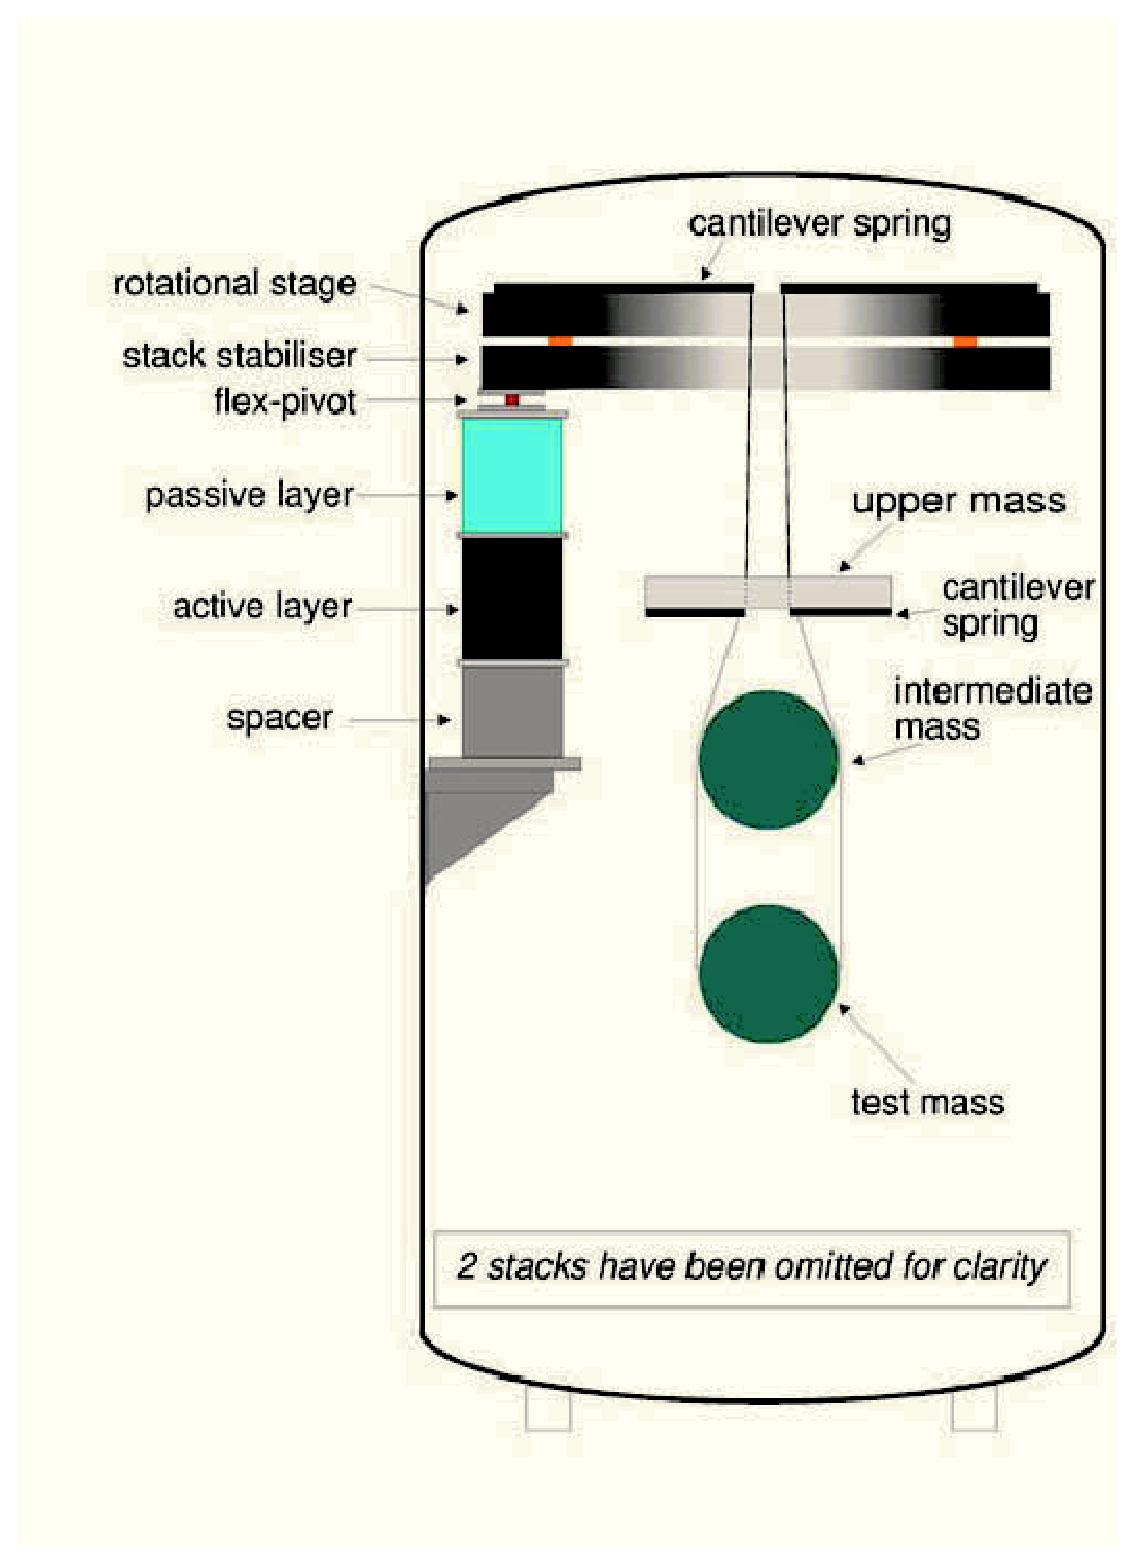
\includegraphics[width=340pt]{figures/fig3/fig3}}
  \caption[]{\label{figure:LIGOseismic}
Internal stages of the large chamber seismic isolation system
for Advanced LIGO (image is inverted for clarity).
}
\end{figure}}

%LivRev: do not use eps for html processing!
\epubtkImage{figures/fig4/fig4.png}{%
\begin{figure}[htbp]
  \centerline{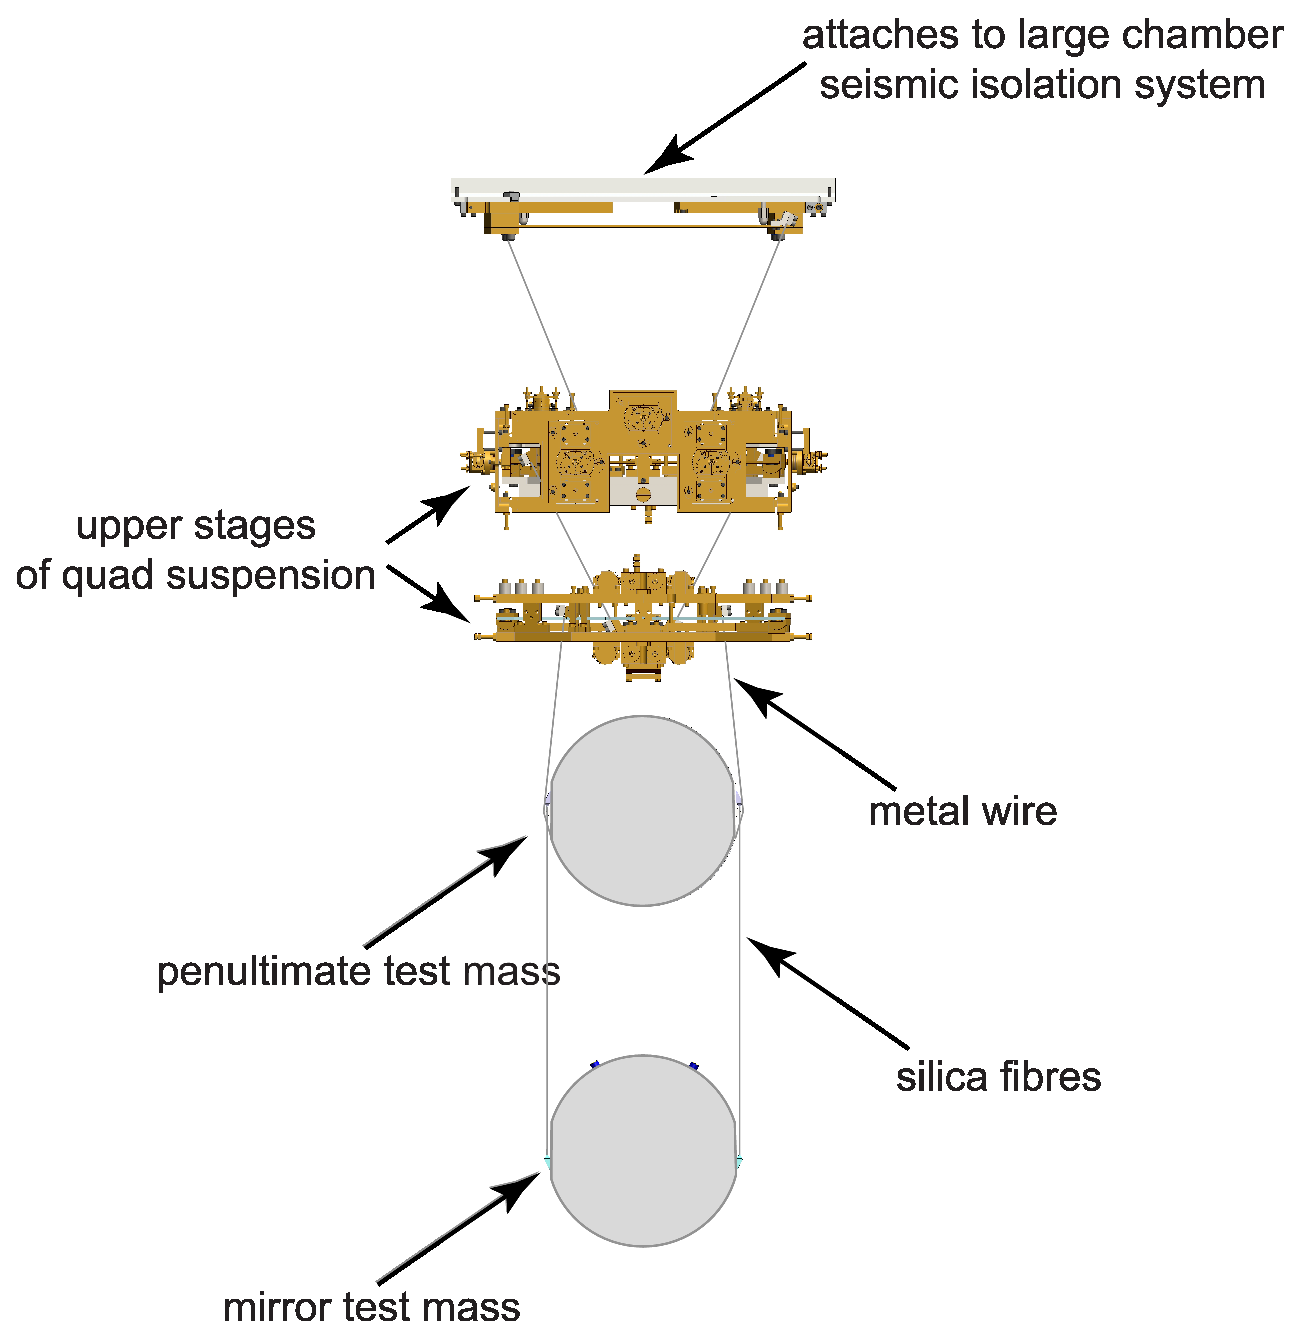
\includegraphics[width=250pt]{figures/fig4/fig4_small}}
  \caption[]{\label{figure:LIGOsens}
Measured sensitivity of the initial LIGO interferometers
    during the S5 science run (see
    Section~\ref{sec:ligoruns}). Reproduced with permission from
    \cite{LIGOcurves}.}
\end{figure}}

\input{Section4_2}

\epubtkImage{figures/GGN/GGN.png}{%
\begin{figure}[htbp]
  \centerline{\includegraphics[width=\textwidth]{figures/GGN/GGN}}
  \caption[]{Time-lapsed schematic illustrating the fluctuating
    gravitational force on a suspended mass by the propagation of a
    surface wave through the ground.}
\end{figure}}


The magnitude of the rms motion of the interferometer test masses,
$\tilde{x}(\omega)$, can be shown to be~\cite{Thorne:1998}
\begin{equation}
  \tilde{x}(\omega) = \frac{4 \pi G \rho}{\omega^{2}} \beta(\omega)
\tilde{W}(\omega),
  \label{equation:GGN}
\end{equation}
where $\rho$ is the Earth's density near the test mass, $G$ is
Newton's constant, $\omega$ is the angular frequency of the seismic
spectrum, $\beta(\omega)$ is a dimensionless reduced transfer function
that takes into account the correlated motion of the interferometer
test masses in addition to the reduction due to the separation between
the test mass and the Earth's surface, and $\tilde{W}(\omega)$ is the
displacement rms-averaged over 3-dimensional directions. In order to
eliminate noise arising from gravity gradients, a detector would have
to be operated far from these density fluctuations, that is, in space.
Proposed space missions are discussed in Section~\ref{section:space}.


However, there are two proposed approaches for reducing the level of gravity-gradient noise in future ground-based detectors. A monitor and subtraction
method can be used, where an array of seismometers can be distributed
strategically around each test mass to monitor the relevant ground motion (and
ground compression) that would be expected to couple through local gravity. A
subtraction signal may be developed from knowing how the observed density
fluctuations couple to the motion of each test mass, and can potentially allow a
significant reduction in gravity-gradient noise.


Another approach is to choose a very quiet location, or better still, to also go
underground, as is already going ahead for LCGT~\cite{Miyoki:2005}. Since the
dominant source of gravity-gradient noise is expected to arise from surface
waves on the Earth, the observed gravity-gradient noise will decrease with depth
into the Earth. Current estimates suggest that gravity-gradient noise can be
suppressed down to around 1~Hz by careful site selection and going $\sim$~150~m
underground~\cite{Beker:2011}. The most promising approach (or likely only
approach) to detecting gravitational waves whose frequency is below 1~Hz is to
build an interferometer in space.


\subsection{Thermal noise}
\label{subsection:thermal} 

Thermal noise associated with the mirror masses and the last stage of their
suspensions is the most significant noise source at the low frequency end of the
operating range of initial long baseline gravitational wave
detectors~\cite{Saulson2}. Advanced detector configurations are also expected to
be limited by thermal noise at their most sensitive frequency
band~\cite{Levin, Nakagawa:2002, Harry:2002, Crooks:2002}. Above the operating
range there are the internal resonances of the test masses. The thermal noise in
the operating range comes from the \emph{tails} of these resonant modes. For any
simple harmonic oscillator such as a mass hung on a spring or hung as a pendulum,
the spectral density of thermal motion of the mass can be expressed
as~\cite{Saulson2}
\begin{equation}
  x^{2}(\omega) = \frac{4 k_{\mathrm{B}} T \omega_{0}^{2}
  \phi(\omega)}{\omega m [{(\omega_{0}^{2} - \omega^{2})^2 +
  \omega_{0}^{4} \phi^{2}(\omega)}]},
  \label{equation:thnoise}
\end{equation}
where $k_{\mathrm{B}}$ is Boltzmann's constant, $T$ is the temperature, $m$ is the
mass and  $\phi(\omega)$ is the loss angle or loss factor of the
oscillator of angular resonant frequency $\omega_0$. This loss factor is the
phase lag angle between the displacement of the mass and any force applied to
the mass at a frequency well below $\omega_0$. In the case of a mass on a spring,
the loss factor is a measure of the mechanical loss associated with the material
of the spring. For a pendulum, most of the energy is stored in the lossless
gravitational field. Thus, the loss factor is lower than that of the material,
which is used for the wires or fibres used to suspend the pendulum. Indeed,
following Saulson~\cite{Saulson2} it can be shown that for a pendulum of mass
$m$, suspended on four wires or fibres of length $l$, the loss factor of the
pendulum is related to the loss factor of the material by
\begin{equation}
  \phi_{\mathrm{pend}}(\omega) = \phi_{\mathrm{mat}}(\omega)\frac{4 \sqrt{TEI}}{mgl},
  \label{equation:pend}
\end{equation}
where $I$ is the moment of the cross-section of  each wire, and $T$ is the
tension in each wire, whose material has a Young's modulus $E$. In general, for
most materials, it appears that the intrinsic loss factor is essentially
independent of frequency over the range of interest for gravitational-wave
detectors (although care has to be taken with some materials in that a form of
damping known as thermo-elastic damping can become important for wires of small
cross-section~\cite{Nowick} and for some bulk crystalline
materials~\cite{Bragthermo}). In order to estimate the internal thermal noise of
a test mass, each resonant mode of the mass can be regarded as a harmonic
oscillator. When the detector operating range is well below the resonances of
the masses, following Saulson~\cite{Saulson2}, the effective spectral density of
thermal displacement of the front face of each mass can be expressed as the
summation of the motion of the various mechanical resonances of the mirror as
also discussed by Gillespie and Raab~\cite{Gillespie}. However, this intuitive
approach to calculating the thermally-driven motion is only valid when the
mechanical loss is distributed homogeneously and, therefore, not valid for real
test-mass mirrors. The mechanical loss is known to be inhomogeneous due to, for
example, the localisation of structural defects and stress within the bulk
material, and the mechanical loss associated with the polished surfaces is
higher than the levels typically associated with bulk effects.  Therefore, Levin
suggested using a direct application of the fluctuation-dissipation theorem to
the optically-sensed position of the mirror substrate surface~\cite{Levin}.
This technique imposes a notional pressure (of the same spatial profile as the
intensity of the sensing laser beam) to the front face of the substrate and
calculates the resulting power dissipated in the substrate on its elastic
deformation under the applied pressure.  Using such an approach we find that
$S_x(f)$ can then be described by the relation
\begin{equation}
 S_x(f) = \frac{2k_\mathrm{B}T}{\pi^2 f^2} \frac{W_{\mathrm{diss}}}{F_0^2},
 \label{eqn:S-x_Levin}
\end{equation}
where $F_0$ is the peak amplitude of the notional oscillatory force and
$W_{\mathrm{diss}}$ is the power dissipated in the mirror described
as,
\begin{equation}
 W_{\mathrm{diss}} = \omega \int{\epsilon(r)\phi(r)\partial V},
 \label{eqn:S-x_Levin2}
\end{equation}
where $\epsilon(r)$ and $\phi(r)$ are the strain and mechanical loss located at
specific positions within the volume $V$. This formalisation highlights the
importance of where mechanical dissipation is located with respect to the
sensing laser beam.  In particular, the thermal noise associated with the
multi-layer dielectric mirror coatings, required for high reflectivity, will in
fact limit the sensitivity of second-generation gravitational-wave detectors at
their most sensitive frequency band, despite these coatings typically being only
$\sim$~4.5~\mum in thickness~\cite{Harry:2002}. Identifying coating
materials with lower mechanical loss, and trying to understand the sources of
mechanical loss in existing coating materials, is a major R\&D effort targeted
at enhancements to advanced detectors and for third generation
instruments~\cite{Martin:2008}.


In order to keep thermal noise as low as possible the mechanical loss factors of
the masses and pendulum resonances should be as low as possible. Further, the
test masses must have a shape such that the frequencies of the internal
resonances are kept as high as possible, must be large enough to accommodate the
laser beam spot without excess diffraction losses, and must be massive enough to
keep the fluctuations due to radiation pressure at an acceptable level. Test
masses currently range in mass from 6~kg for GEO600 to 40~kg for Advanced LIGO.
To approach the best levels of sensitivity discussed earlier the loss factors of
the test masses must be $\simeq$~3~\texttimes~10\super{-8} or lower,
and the loss factor of the pendulum resonances should be smaller than
10\super{-10}.


Obtaining these values puts significant constraints on the choice of material
for the test masses and their suspending fibres. GEO600 utilises very-low--loss
silica suspensions, a technology, which should allow detector sensitivities to
approach the level desired for second generation instruments~\cite{Braginsky1,
Rowan1, Rowan2}, since the intrinsic loss factors in samples of synthetic fused
silica have been measured down to around
5~\texttimes~10\super{-9}~\cite{Ageev:2004}. Still, the use of other
materials such as sapphire is being seriously considered for future
detectors~\cite{Braginsky2, Ju2, Rowan1} such as in
LCGT~\cite{Miyoki:2005, Ohashi:2008}.


The technique of hydroxy-catalysis bonding provides a method of jointing oxide
materials in a suitably low-loss way to allow `monolithic' suspension systems to
be constructed~\cite{Rowan3}. A recent discussion on the level of mechanical
loss and the associated thermal noise in advanced detectors resulting from
hydroxy-catalysis bonds is given by Cunningham et al.~\cite{Cunningham:2010}.
Images of the GEO600 monolithic mirror suspension and of the prototype Advanced
LIGO mirror suspension are shown in Figure~\ref{figure:monolithic}.


%LivRev: do not use eps for html processing!
\epubtkImage{figures/monolithic/monolithic.png}{%
\begin{figure}[htbp]
  \centerline{\includegraphics[width=\textwidth]{figures/monolithic/monolithic_small}}
  \caption[]{\label{figure:monolithic}
Monolithic silica suspension of (a) GEO600 6~kg mirror test mass
suspended from 4 fibres of thickness 250~\mum and (b) prototype monolithic
suspension for Advanced LIGO at LASTI (mirror mass of 40~kg, silica fibre
thickness 400~\mum).
}
\end{figure}}

\input{Section4_4}

%\newpage

\input{Section5_1}

\epubtkImage{figures/fig5e/fig5e.png}{%
\begin{figure}[htbp]
  \centerline{\includegraphics[width=\textwidth]{figures/fig5e/fig5e}}
  \caption[]{Michelson interferometers with (a) delay lines and (b)
Fabry--P\'{e}rot cavities in the arms of the interferometer.}
\end{figure}}

Optimally, the light should be stored for a time comparable to the
characteristic timescale of the signal. Thus, if signals of characteristic
timescale 1~msec are to be searched for, the number of bounces should be
approximately 50 for an arm length of 3~km. With 50 bounces the required laser
power is reduced to 2.4~\texttimes~10\super{3}~W, still a formidable
requirement.


\subsection{Power recycling}
\label{subsection:powerrec} 

It can be shown that an optimum signal-to-noise ratio in a Michelson interferometer
can be obtained when the arm lengths are such that the output light is very
close to a minimum (this is not intuitively obvious and is discussed more fully
in~\cite{Edelstein}). Thus, rather than lock the interferometer to the side of a
fringe as discussed above in Section~\ref{subsubsection:shotnoise}, it is usual
to make use of a modulation technique to operate the interferometer close to a
null in the interference pattern. An electro-optic phase modulator placed in
front of the interferometer can be used to phase modulate the input laser light.
If the arms of the interferometer are arranged to have a slight mismatch in
length this results in a detected signal, which, when demodulated, is zero with
the cavity exactly on a null fringe and changes sign on different sides of the
null providing a bipolar error signal; this can be fed back to the transducer
controlling the interferometer mirror to hold the interferometer locked near to
a null fringe (this is the RF readout scheme discussed in Section~\ref{sec:readout}).


In this situation, if the mirrors are of very low optical loss, nearly all of the
light supplied to the interferometer is reflected back towards the laser. In
other words the laser is not properly impedance matched to the interferometer.
The impedance matching can be improved by placing another mirror of correctly
chosen transmission -- a power recycling mirror -- between the laser and the
interferometer so that a resonant cavity is formed between this mirror and the
rest of the interferometer; in the case of perfect impedance matching, no light
is reflected back towards the laser~\cite{Drever3, Schilling}. There is then a
power build-up inside the interferometer as shown in 
Figure~\ref{figure:Michelsons2a}. This can be high enough to create the required
kilowatts of laser light at the beamsplitter, starting from an input laser light
of only about 10~W.


\epubtkImage{figures/fig6a/fig6a.png}{%
\begin{figure}[htbp]
  \centerline{\includegraphics[width=0.5\textwidth]{figures/fig6a/fig6a}}
  \caption[]{\label{figure:Michelsons2a}
The implementation of power recycling on a
    Michelson interferometer with Fabry--P\'{e}rot cavities.
}
\end{figure}}


To be more precise, if the main optical power losses are those associated with
the test mass mirrors -- taken to be A per reflection -- the intensity inside
the whole system considered as one large cavity is increased by a factor given
by $(\pi L)/(c A \tau)$, where the number of bounces, or light storage time, is
optimised for signals of timescale $\tau$ and the other symbols have their usual
meaning. Then:
\begin{equation}
  \mathrm{detectable\ strain\ in\ time\ } \tau = \left( \frac{\lambda h
  A}{4 \pi L P \tau^2} \right)^{1/2}.
  \label{equation:shotpower}
\end{equation}


\subsection{Signal recycling}
\label{subsection:sigrec} 

To enhance further the sensitivity of an interferometric detector and to allow
some narrowing of the detection bandwidth, which may be valuable in searches for
continuous wave sources of gravitational radiation, another technique known as
signal recycling can be implemented~\cite{Meers, Strain, Heinzel}. This relies
on the fact that sidebands created on the light by gravitational-wave signals
interacting with the arms do not interfere destructively and so do appear at the
output of the interferometer. If a mirror of suitably-chosen reflectivity is put
at the output of the system as shown in Figure~\ref{figure:Michelsons2b}, then the
sidebands can be recycled back into the interferometer, where they resonate, and
hence the signal size over a given bandwidth (set by the mirror reflectivity) is
enhanced.


\epubtkImage{figures/fig6b/fig6b.png}{%
\begin{figure}[htbp]
  \centerline{\includegraphics[width=0.5\textwidth]{figures/fig6b/fig6b}}
  \caption[]{The implementation of signal recycling on a
    Michelson interferometer with Fabry--P\'{e}rot cavities.}
\end{figure}}

\input{Section5_4}

\newpage

\input{Section6_1}

\epubtkImage{figures/figpro/figpro.png}{%
\begin{figure}[htbp]
  \centerline{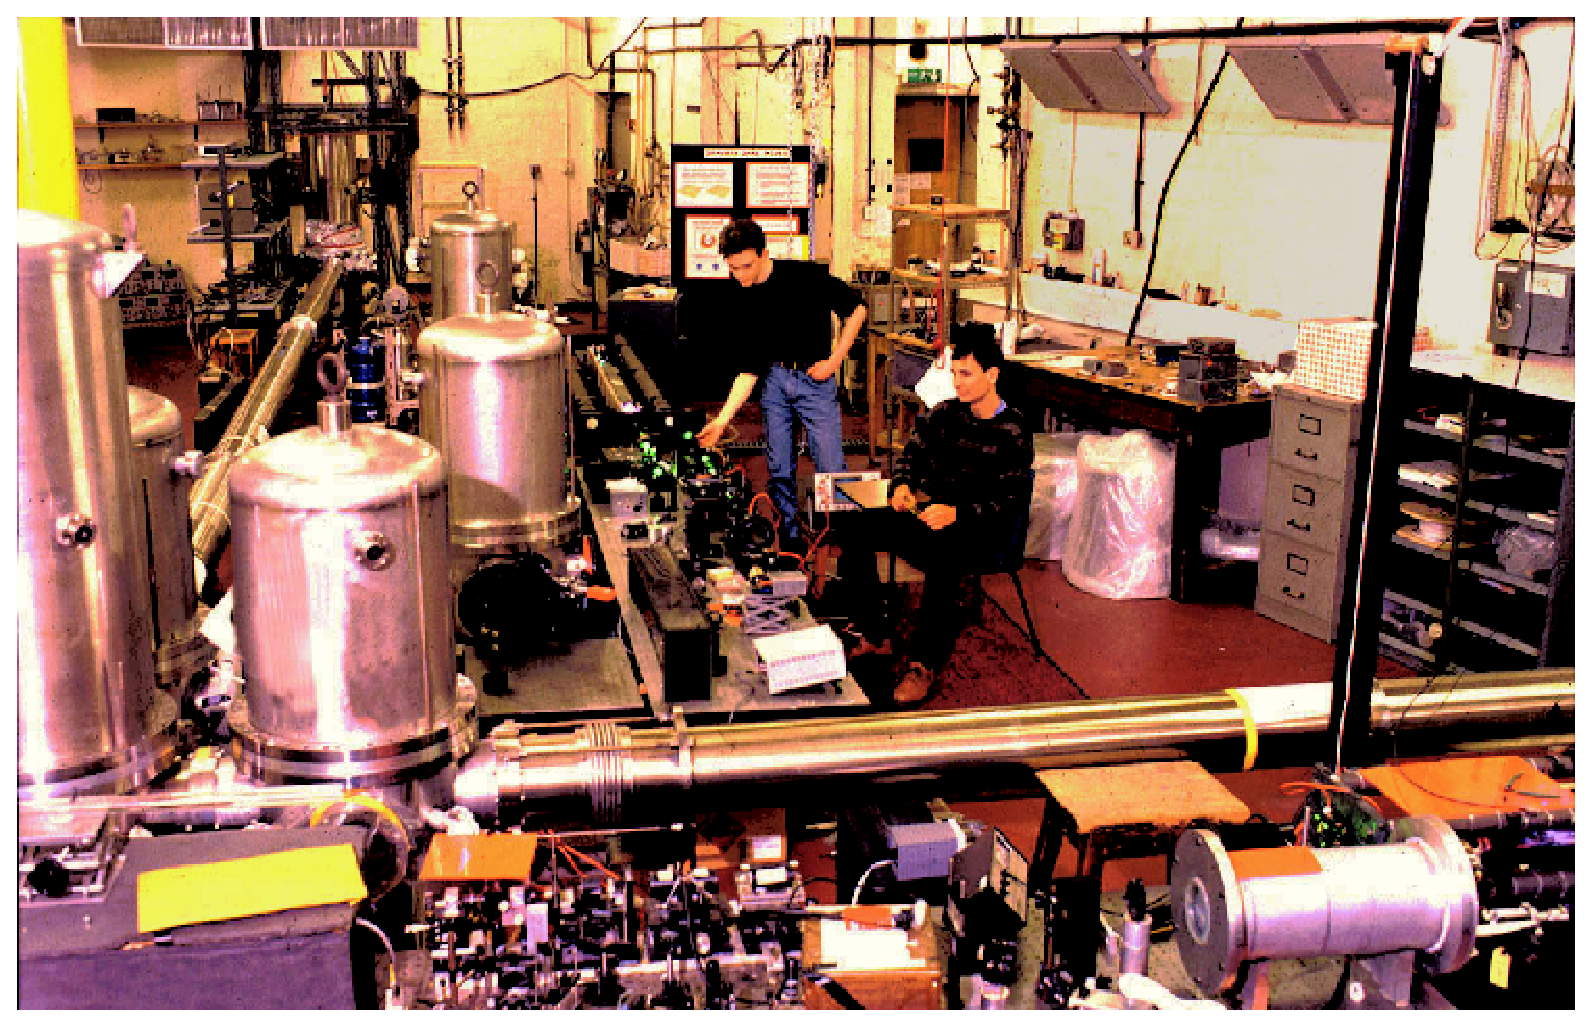
\includegraphics[scale=0.4]{figures/figpro/figpro}}
  \caption[]{The 10~m prototype gravitational wave detector
    at Glasgow.}
\end{figure}}

The sensitivities of some of these detectors reached a level -- better than
10\super{-18} for millisecond bursts -- such that the technology could be
considered sufficiently mature to propose the construction of detectors of much
longer baseline that would be capable of reaching the performance required to
have a real possibility of detecting gravitational waves.  An international
network of such long baseline gravitational wave detectors has now been
constructed and commissioned, and science-quality data from these has been
produced and analysed since 2002 (see Section~\ref{subsection:runs} and
Section~\ref{subsection:results} for a review of recent science data runs and
results).


The American LIGO project~\cite{LIGOweb} comprises two detector systems with
arms of 4~km length, one in Hanford, Washington, and one in Livingston,
Louisiana (also known as the LIGO Hanford Observatory 4k [LHO~4k] and LIGO
Livingston Observatory 4k [LLO~4k], or H1 and L1, respectively). One half length,
2~km, interferometer was also contained inside the same evacuated enclosure at
Hanford (also known as the LHO~2k, or H2). The design goal of the 4~km
interferometers was to have a peak strain sensitivity between 100\,--\,200~Hz of
$\sim$~3~\texttimes~10\super{-23}~\Hz~\cite{LIGOSRD} (see
Figure~\ref{figure:LIGOstrains}), which was achieved during the fifth science run
(Section~\ref{subsection:runs}). A birds-eye view of the Hanford site showing the
central building and the directions of the two arms is shown in
Figure~\ref{figure:LIGOsite}. In October 2010 the LIGO detectors shut down and
decommissioning began in preparation for the installation of a more sensitive
instrument known as Advanced LIGO (see Section~\ref{subsection:aligo}).


\epubtkImage{figures/fig7/fig7.png}{%
\begin{figure}[htbp]
  \centerline{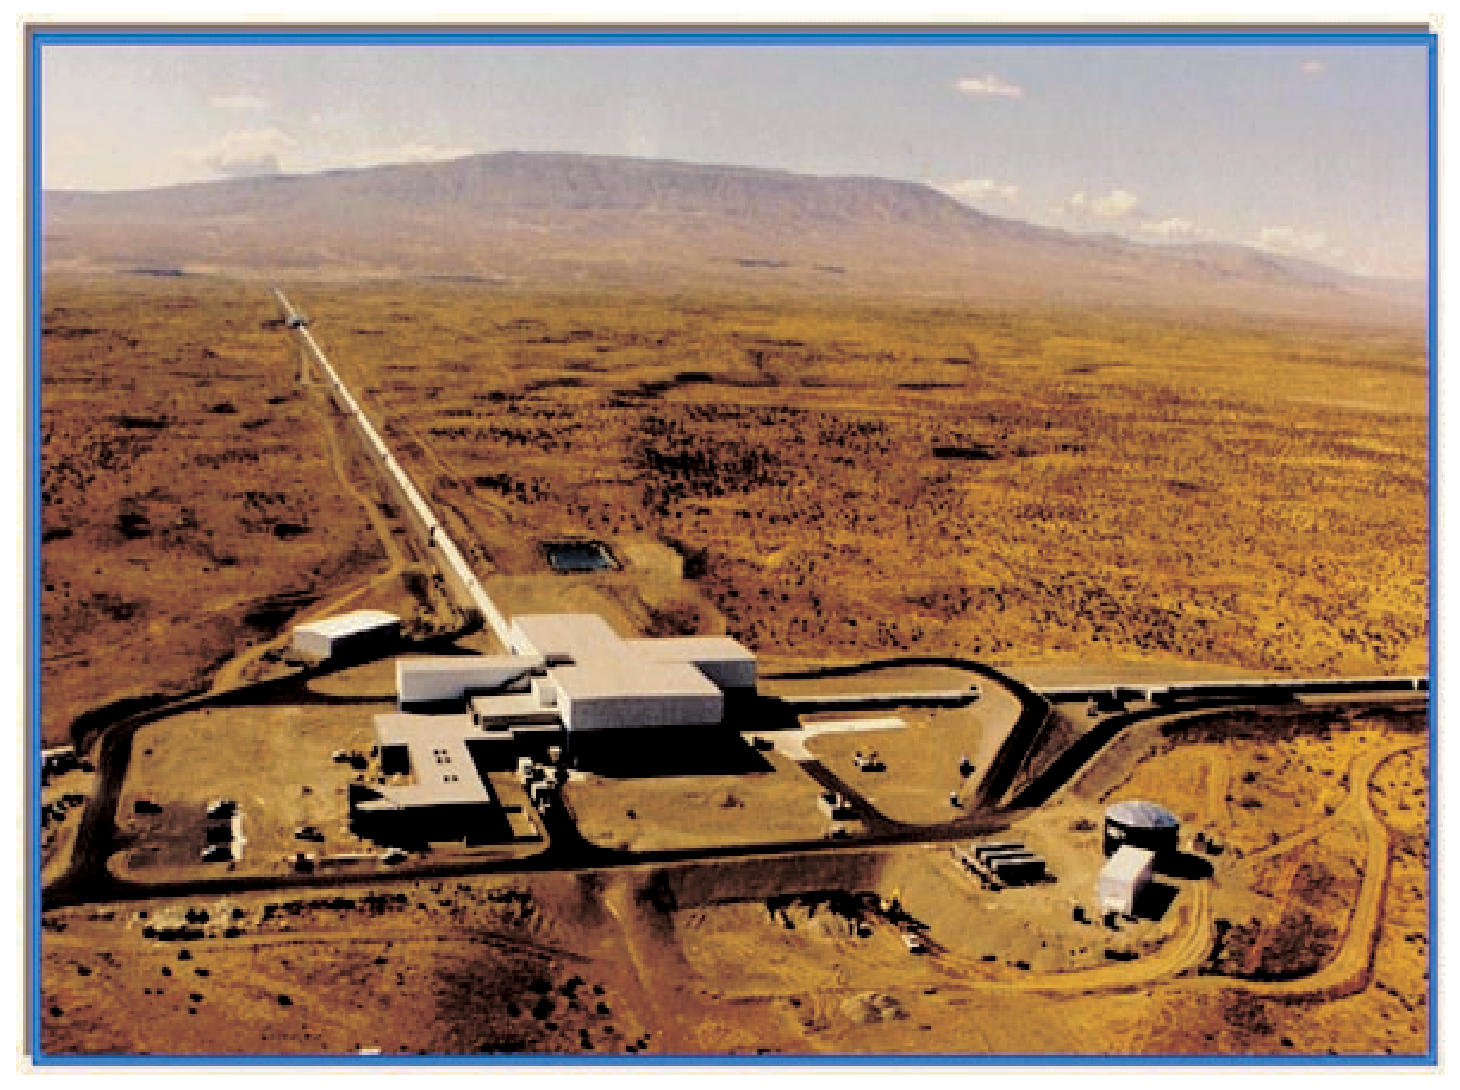
\includegraphics[width=12cm]{figures/fig7/fig7}}
  \caption[]{\label{figure:LIGOsite}
A bird's eye view of the LIGO detector, sited in
    Hanford, Washington.
}
\end{figure}}

The French/Italian Virgo project~\cite{VIRGOweb} comprises a single
3~km arm-length detector at Cascina near Pisa. As mentioned earlier,
it is designed to have better performance than the other detectors,
down to 10~Hz.

The TAMA300 detector~\cite{TAMAweb}, which has arms of length 300~m, at the
Tokyo Astronomical Observatory was the first of the ``beyond-prototype''
detectors to become operational. This detector is built mainly underground and
partly has the aim of adding to the gravitational-wave detector network for
sensitivity to events within the local group of galaxies, but is primarily a
test bed for developing techniques for future larger-scale detectors. Initial
operation of the interferometer was achieved in 1999 and power recycling was
implemented for data taking in 2003~\cite{Arai:2003}.

All the systems mentioned above are designed to use resonant cavities in the
arms of the detectors and use standard wire-sling techniques for suspending the
test masses. The German/British detector, GEO600~\cite{GEOweb}, built near
Hannover, Germany, is somewhat different. It makes use of a four-pass delay-line
system with advanced optical signal-enhancement techniques, utilises very-low
loss-fused silica suspensions for the test masses, and, despite its smaller size,
was designed to have a sensitivity at frequencies above a few hundred Hz
comparable to the first phases of Virgo and LIGO during their initial operation.
It uses both power recycling (Section~\ref{subsection:powerrec}) and tunable signal
recycling (Section~\ref{subsection:sigrec}), often referred to together as dual
recycling.


To gain the most out of the detectors as a true network, data sharing and joint
analyses are required. In the summer of 2001 the LIGO and GEO600 teams signed a
Memorandum of Understanding (MoU), under the auspices of the LIGO Scientific
Collaboration (LSC)~\cite{LSCweb}, allowing complete data sharing between the
two groups. Part of this agreement has been to ensure that both LIGO and
GEO600 have taken data in coincidence (see below). Coincident data taking, and
joint analysis, has also occurred between the TAMA300 project and the LSC
detectors. The Virgo collaboration also signed an MoU with the LSC, which has
allowed data sharing since May 2006.


The operation and commissioning of these detectors is a continually-evolving
process, and the current state of this review only covers developments until
late-2010. For the most up-to-date information on detectors readers are advised
to consult the proceedings of the Amaldi meetings, GWDAW/GWPAW (Gravitational
Wave Data Analysis Workshops), and GWADW (Gravitational Wave Advanced Detectors
Workshops) -- see~\cite{confs} for a list of past conferences.


For the first and second generations of detector, much effort has gone into
estimating the expected number of sources that might be observable given their
design sensitivities. In particular, for what are thought to be the strongest
sources: the coalescence of neutron-star binaries or black holes (see
Section~\ref{sec:cbc} for current rates as constrained by observations). These
estimates, based on observation and simulation, are summarised in
Table~5 of~\cite{Abadie:2010e} and the \textit{realistic} rates
suggest initial detectors would expect to see 0.02, 0.004 and 0.007
events per year for neutron-star--binary, black-hole--neutron-star, and
black-hole--binary systems, respectively (it should be noted that there
is a range of possible rates consistent with current observations and
models)\epubtkFootnote{In terms of event rates the current best estimates
for neutron-star--binary merger rates, based on the known population
of neutron-star--binary systems, gives a 95\% confidence interval
between 1\,--\,1000~\texttimes~10\super{-6} per year per Milky Way
Equivalent Galaxy (MWEG), where MWEG is equivalent to a volume that
contains a blue light luminosity with $L = 9\times10^9\,L_{\odot}$
(MWEG was used in the S1 and S2 LIGO search, but was then changed to
the $L_{10}$ unit, where $L_{10}$ is given as 10\super{10} times the
blue-light luminosity of the sun, although there is only a 10\%
difference between the two),~\cite{Abadie:2010e, Kalogera:2004a,
Kalogera:2004b}, with a peak in the distribution at
100~\texttimes~10\super{-6} per year per MWEG -- or $\approx$~0.02 per year
for initial LIGO at design sensitivity. The expected rate of black-hole binary systems, or black-hole--neutron-star systems is far harder
to infer as none have been observed, but estimates can be made on
the population for a wide variety of models and give a 95\%
confidence range of 0.05\,--\,100~\texttimes~10\super{-6} per year per
MWEG and 0.01\,--\,30~\texttimes~10\super{-6} per year per MWEG
respectively~\cite{Abadie:2010e, OShaughnessy:2005,
OShaughnessy:2008, Abbott:2008a}. As an example of how to convert
from rates to event numbers, cumulative blue-light luminosities with
respect to distance from the Earth in Mpcs, and the horizon
distances of the LIGO detectors from S2 through to S4, can be seen
in Figure~3 of~\cite{Abbott:2008a}.}. Second generation detectors
(see Section~\ref{subsection:aligo}), which can observe approximately
1000 time more volume than the initial detectors might, expect to see
40, 10, and 20 per year for the same sources. With such rates a great
deal of astrophysics could be possible (see~\cite{Sathyaprakash:2009}
for examples).


\subsection{Science runs}
\label{subsection:runs} 

Over the last decade the commissioning and improvement of the various
gravitational-wave detectors has been suspended at various stages to take data
for astrophysical analysis. These have been times when it was considered that
the detectors were sensitive and stable enough (or had made sufficient
improvements over earlier states) to make astrophysical searches worthwhile.
Within the LSC these have been called the \textit{Science} (S) runs, for Virgo they
have been the \textit{Virgo Science Runs} (VSR), and for TAMA300 they have been
the \textit{Data Taking} (DT) periods. A time-line of science runs for the various
interferometric detectors, can be seen in Figure~\ref{figure:runtimes}.

\epubtkImage{figures/runtimes/runtimes.png}{%
\begin{figure}[htbp]
  \centerline{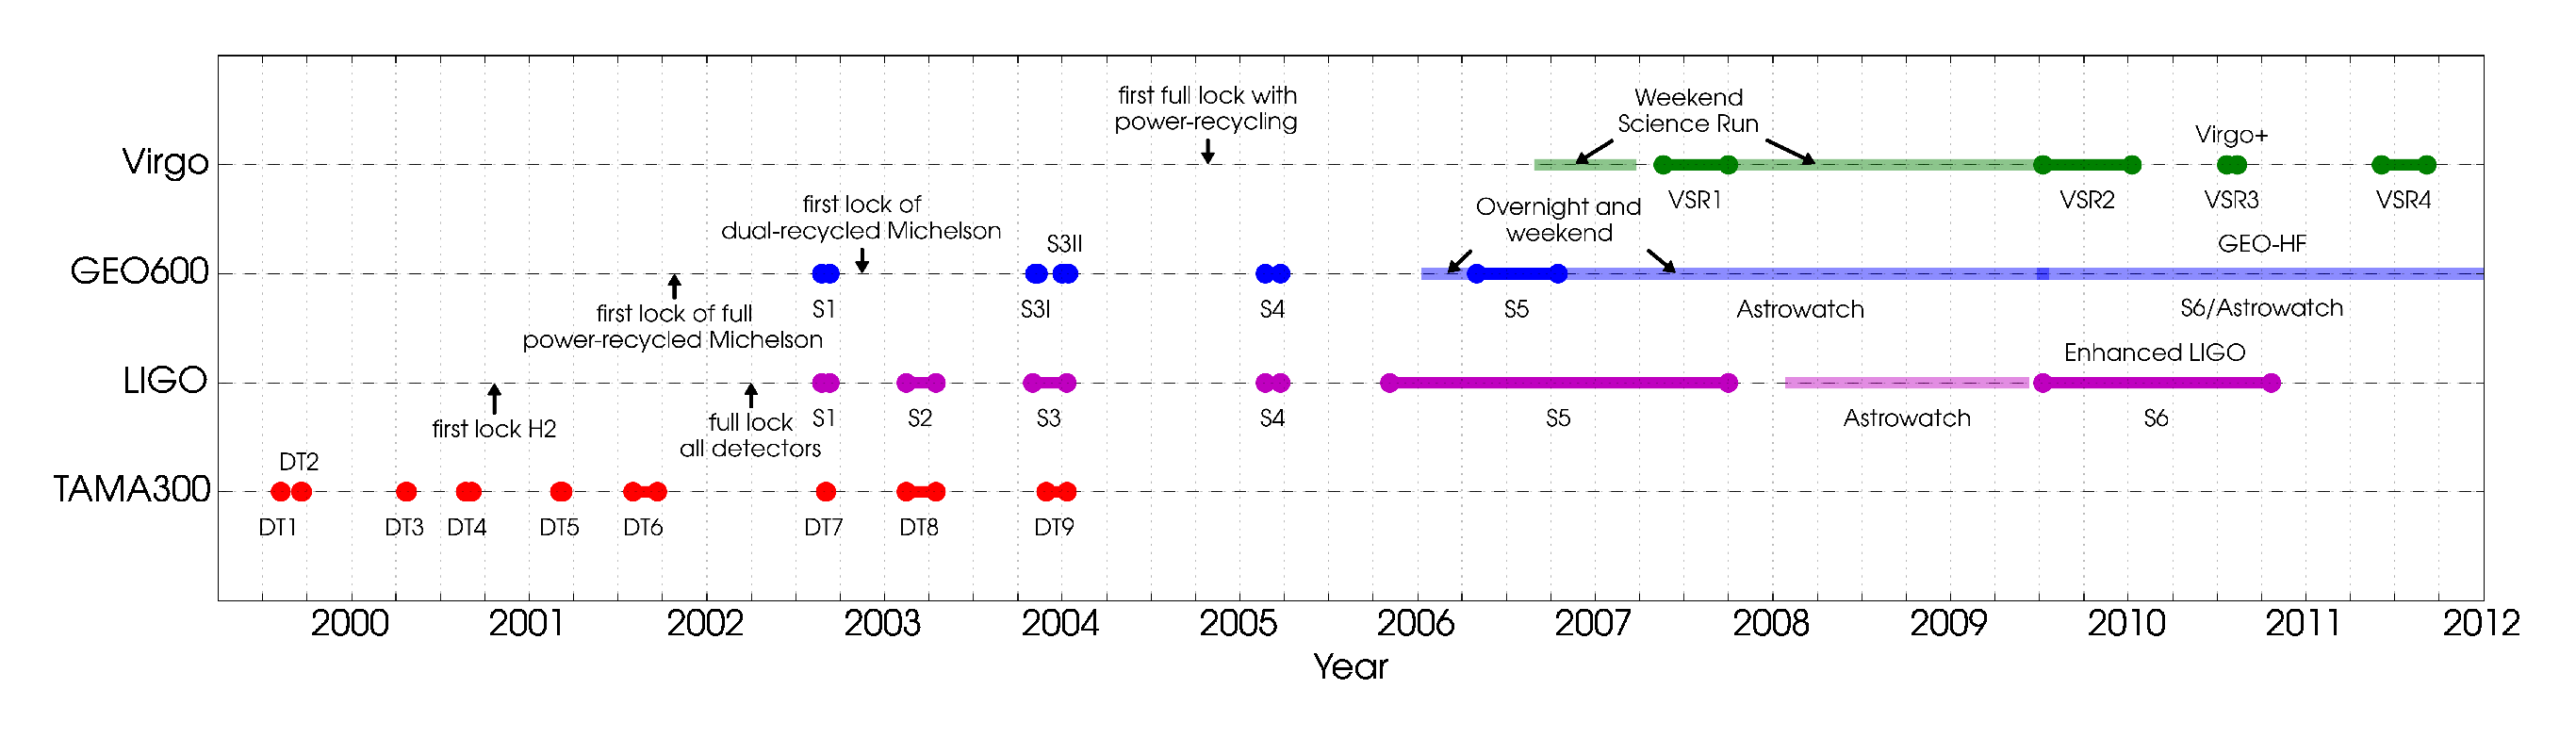
\includegraphics[width=\textwidth]{figures/runtimes/runtimes}}
  \caption[]{\label{figure:runtimes}
A time-line of the science runs of the first generation interferometric gravitational-wave detectors, from their first lock to mid-2011 (the `initial detector era'). This timeline ends before the Virgo VSR4 run in June to September 2011.
}
\end{figure}}

A figure of merit for the sensitivity of a detector is to calculate
its \textit{horizon distance}. This is the maximum range out to which
it could see the coalescence of two $1.4\,M_{\odot}$ neutron stars
that are optimally oriented and located (i.e., with the orbital plane
perpendicular to the line-of-sight, and with this plane parallel to
the detector plane, so that the antenna response is at its maximum) at
a signal-to-noise ratio of 8~\cite{Abbott:2005b}. The horizon distance
can be converted to a range that is an average over all sky locations
and source orientations (i.e.\, not the best case scenario) by dividing
it by 2.26~\cite{Sutton:2003}) -- we shall use this angle averaged
range throughout the rest of this review.

\subsubsection{TAMA300}


The first interferometric detector to start regular data taking with sufficient
sensitivity and stability to enable it to potentially detect gravitational waves
from the the galactic centre was TAMA300~\cite{Ando:2001}. Over the period
between August 1999 to January 2004 TAMA had nine data-taking periods
(denominated DT1--9) over which time its typical strain noise sensitivity, in
its most sensitive frequency band improved from
$\sim$~3~\texttimes~10\super{-19}~\Hz to
$\sim$~1.5~\texttimes~10\super{-21}~\Hz~\cite{Akutsu:2006}. TAMA300
operated in coincidence with the LIGO and GEO600 detectors for two of
the science data-taking periods. More recently focus has shifted to
the Cryogenic Laser Interferometer Observatory (CLIO) prototype
detector~\cite{Yamamoto:2008, CLIOweb}, designed to test technologies
for a future \textit{second-generation} Japanese detector called the
Large-scale Cryogenic Gravitational-Wave Telescope (LCGT) (see
Section~\ref{subsection:aligo}).


\subsubsection{LIGO}
\label{sec:ligoruns} 

The first LIGO detector to achieve lock (meaning having the interferometer
stably held on a dark fringe of the interference pattern, with light resonating
throughout the cavity) was H2 in late 2000. By early 2002 all three detectors
had achieved lock and have since undergone many periods of commissioning and
science data taking. Over the period from mid-2001 to mid-2002 the
commissioning process improved the detectors' peak sensitivities by several
orders of magnitude, with L1 going from
$\sim$~10\super{-17}\,--\,10\super{-20}~\Hz at 150~Hz. In summer 2002
it was decided that the detectors were at a sensitivity, and had a
good enough lock stability, to allow a science data-taking run. This
was potentially sensitive to local galactic burst events. From 23
August to 9 September 2002 the three LIGO detectors, along with GEO600
(and, for some time, TAMA300), undertook their first coincident
science run, denoted S1 (see~\cite{Abbott:2004a} for the state of the
LIGO and GEO600 detectors at the time of S1). At this time the most
sensitive detector was L1 with a peak sensitivity at around 300~Hz of
2\,--\,3~\texttimes~10\super{-21}~\Hz. The best strain
amplitude sensitivity curve for S1 (and the subsequent LIGO science runs) can be seen in
Figure~\ref{figure:LIGOstrains}. The amount of time over the run that
the detectors were said to be in science mode, i.e., stable and with
the interferometer locked, called their duty cycle, or duty factor,
was 42\% for L1, 58\% for H1 and 73\% for H2. For the most sensitive
detector, L1, the inspiral range was typically 0.08~Mpc.

% LIGO S1 through S5 best strain sensitivities
\epubtkImage{figures/LIGOSrunASDs/LIGOSrunASDs.png}{%
\begin{figure}[htbp]
  \centerline{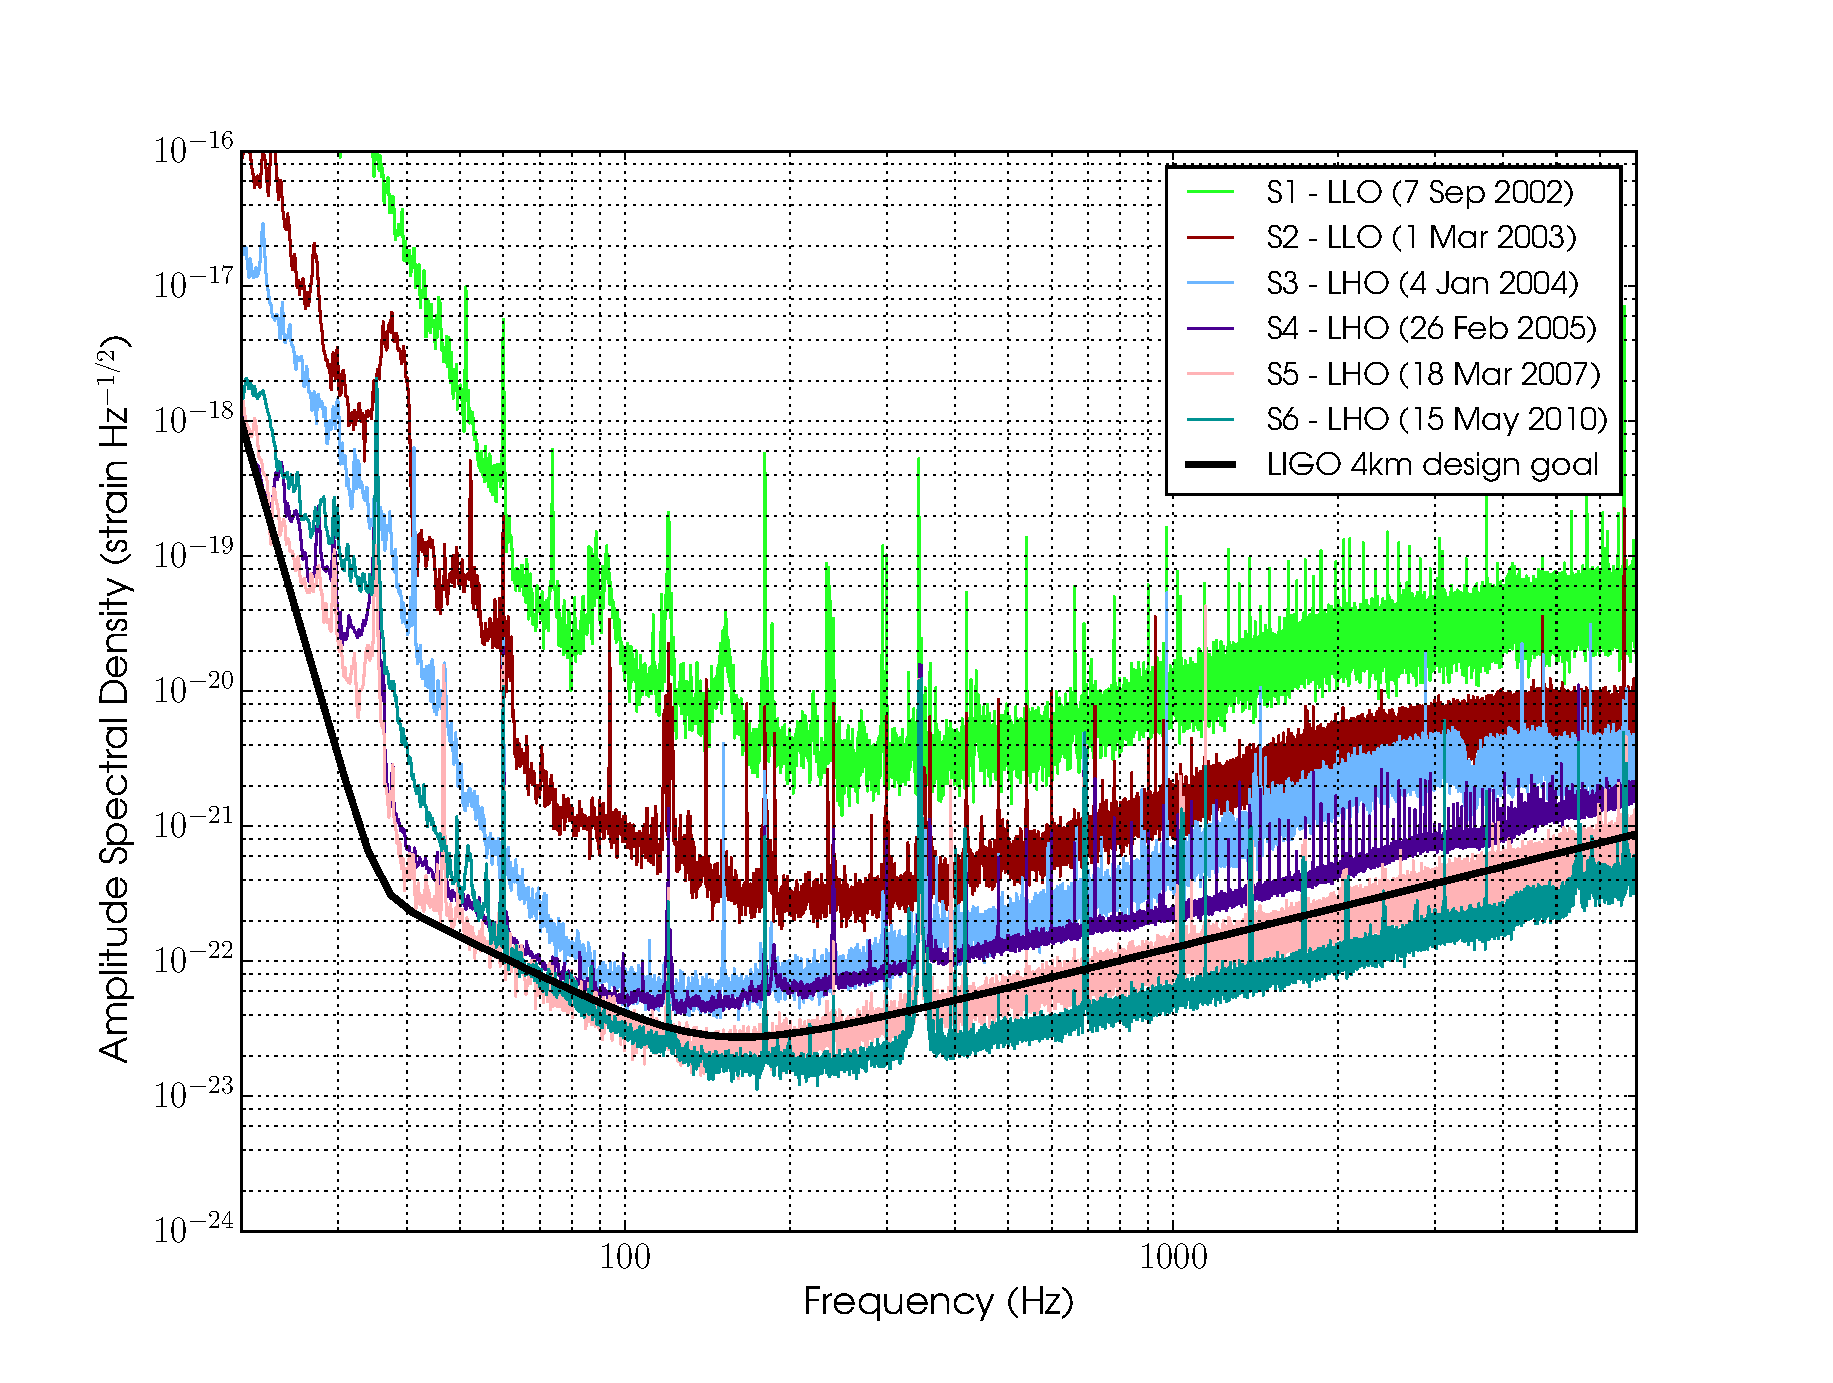
\includegraphics[scale=0.45]{figures/LIGOSrunASDs/LIGOSrunASDs}}
  \caption[]{\label{figure:LIGOstrains}
The best strain sensitivities from the LIGO science runs S1
through S6~\cite{LIGOcurves}. Also shown is the LIGO 4~km design sensitivity.
}
\end{figure}}

For the second science run (S2), from 14 February to 14 April 2003, the noise
floor was considerably improved over S1 by several upgrades including: improving
and stabilising the optical levers used to measure the mirror orientation to
reduce the low frequency ($\lesssim$~50~Hz) noise; replacing the coil drivers
that are used as actuators to control the position and orientation of suspended
mirrors, to improve the mid-frequency ($\sim$~50\,--\,200~Hz) noise floor; and
increasing the laser power in the interferometer to reduce shot noise and
improve the high frequency ($\gtrsim$~200~Hz) sensitivity (see
Section~IIA of~\cite{Abbott:2005a} for a more thorough description of
the detector improvements made for S2). These changes improved the
sensitivities by about an order of magnitude across the frequency band
with a best strain, for L1, of $\sim$~3~\texttimes~10\super{-22}~\Hz
between 200\,--\,300~Hz. The duty factor during S2 was 74\% for H1,
58\% for H2 and 38\% for L1, with a triple coincidence time when all
three detectors were in lock of 22\% of the run. The average inspiral
ranges during the run were approximately 0.9, 0.4 and 0.3~Mpc for L1,
H1 and H2 respectively. This run was also operated in coincidence with
the TAMA300 DT8 run. 


For the the third science run (S3), from 31 October 2003 to 9 January 2004,
the detectors were again improved, with the majority of sensitivity increase in
the mid-frequency range. This run was also operated partially in coincidence
with GEO600. The best sensitivity, which was for H1, was
$\sim$~5~\texttimes~10\super{-23}~\Hz between 100\,--\,200~Hz. The duty factors
were 69\% for H1, 63\% for H2 and only 22\% for L1, with a 16\% triple
coincidence time. L1's poor duty factor was due to large levels of anthropogenic
seismic noise near the site during the day.


The fourth science run (S4), from 22 February to 23 March 2005, saw less-drastic
improvements in detector sensitivity across a wide frequency band, but did make
large improvements for frequencies $\lesssim$~70~Hz. Between S3 and S4 a better
seismic isolation system, which actively measured and countered for ground
motion, was installed in L1, greatly reducing the amount of time it was thrown
out of lock. For H1 the laser power was able to be increased to its full design
power of 10~W~\cite{Abbott:2007b}. The duty factors were 80\% for H1, 81\% for
H2 and 74\% for L1, with a 56\% triple coincidence time. The most sensitive
detector, H1, had an inspiral range of 7.1~Mpc.


By mid-to-late 2005 the detectors had equaled their design sensitivities over
most of the frequency band and were also maintaining good stability and high
duty factors. It was decided to perform a long science run with the aim of
collecting one year's worth of triple coincident data, with an angle-averaged
inspiral range of equal to, or greater than, 10~Mpc for L1 and H1, and 5~Mpc
or better for H2. This run, S5, spanned from 4 November 2005 (L1 started
slightly later on 14 November) until 1 October 2007, and the performance of the
detectors during it is summarised in~\cite{LIGOS5}. One year of triple
coincidence was achieved on 21 September 2007, with a total triple coincidence
duty factor of 52.5\% for the whole run. The average insprial range over S5
was $\sim$~15~Mpc for H1 and L1, and $\sim$~8~Mpc for H2.


After the end of S5 the LIGO H2 detector and GEO600 were kept operational while
possible in an evening and weekend mode called Astrowatch. This observing mode
continued until early 2009, after which H2 was retired. During this time
commissioning of some upgrades to the 4~km LIGO detectors took place for the
sixth and final initial LIGO science run (S6) -- some of which are
summarised in~\cite{Whitcomb:2008}. The aim of these upgrades, called
Enhanced LIGO~\cite{EnhancedLIGO}, was to try and  increase
sensitivity by a factor of two. Enhanced LIGO involved the direct
implementation of technologies and techniques designed for the later
upgrade to Advanced LIGO (see Section~\ref{subsection:aligo}) such as,
most notably, higher-powered lasers, a DC readout scheme (see
Section~\ref{sec:readout}), the addition of output mode cleaners and
the movement of some hardware into the vacuum system. The lasers,
supplied by the Albert Einstein Institute and manufactured by Laser
Zentrum Hannover, give a maximum power of $\approx$~30~W, which is
around 3 times the initial LIGO power. The upgrade to higher power
required that several of the optical components needed to be
replaced. These upgrades were only carried out on the 4~km H1 and L1
detectors due to the H2 detector being left in Astrowatch mode during
the commissioning period. The upgrades were able to produce 1.5\,--\,2
times sensitivity increases at frequencies above $\approx$~200~Hz, but
generally at lower frequencies various sources of noise meant
sensitivity increases were not possible. S6 took place from July 2009
until 20 October 2010, at which point decommissioning started for the
full upgrade to Advanced LIGO. Typically the detectors ran with laser
power at $\approx$~10~W during the day (at higher power the detector
was less stable and the higher level of anthropogenic noise during the
day meant that achieving and maintaining lock required lower power)
and $\approx$~20~W at night, leading to inspiral ranges from
$\approx$~10\,--\,20~Mpc.


\subsubsection{GEO600}


GEO600 achieved first lock as a power-recycled Michelson (with no signal
recycling) in late 2001. Commissioning over the following year,
detailed in~\cite{Hewitson:2003}, included increases in the laser
power, installation of monolithic suspensions for the end test masses
(although not for the beam splitter and inboard mirrors),
rearrangement of the optical bench to reduce scattered light and
implementation of an automatic alignment system. For the S1 run,
carried out in coincidence with LIGO (and, in part, TAMA300), the
detector was kept in this configuration (see~\cite{Abbott:2004a} for
the status of the detector during S1). It had a very high duty factor
of $\sim$~98\%, although its strain sensitivity was $\sim$~2 orders of
magnitude lower than the LIGO instruments. The auto-alignment system
in GEO600 has since meant that it has been able to operate for long
periods without manual intervention to regain lock, as has been the
case for initial LIGO.

% GEO S1 through S5 typical strain sensitivities
\epubtkImage{figures/GEOSrunASDs/GEOSrunASDs.png}{%
\begin{figure}[htbp]
  \centerline{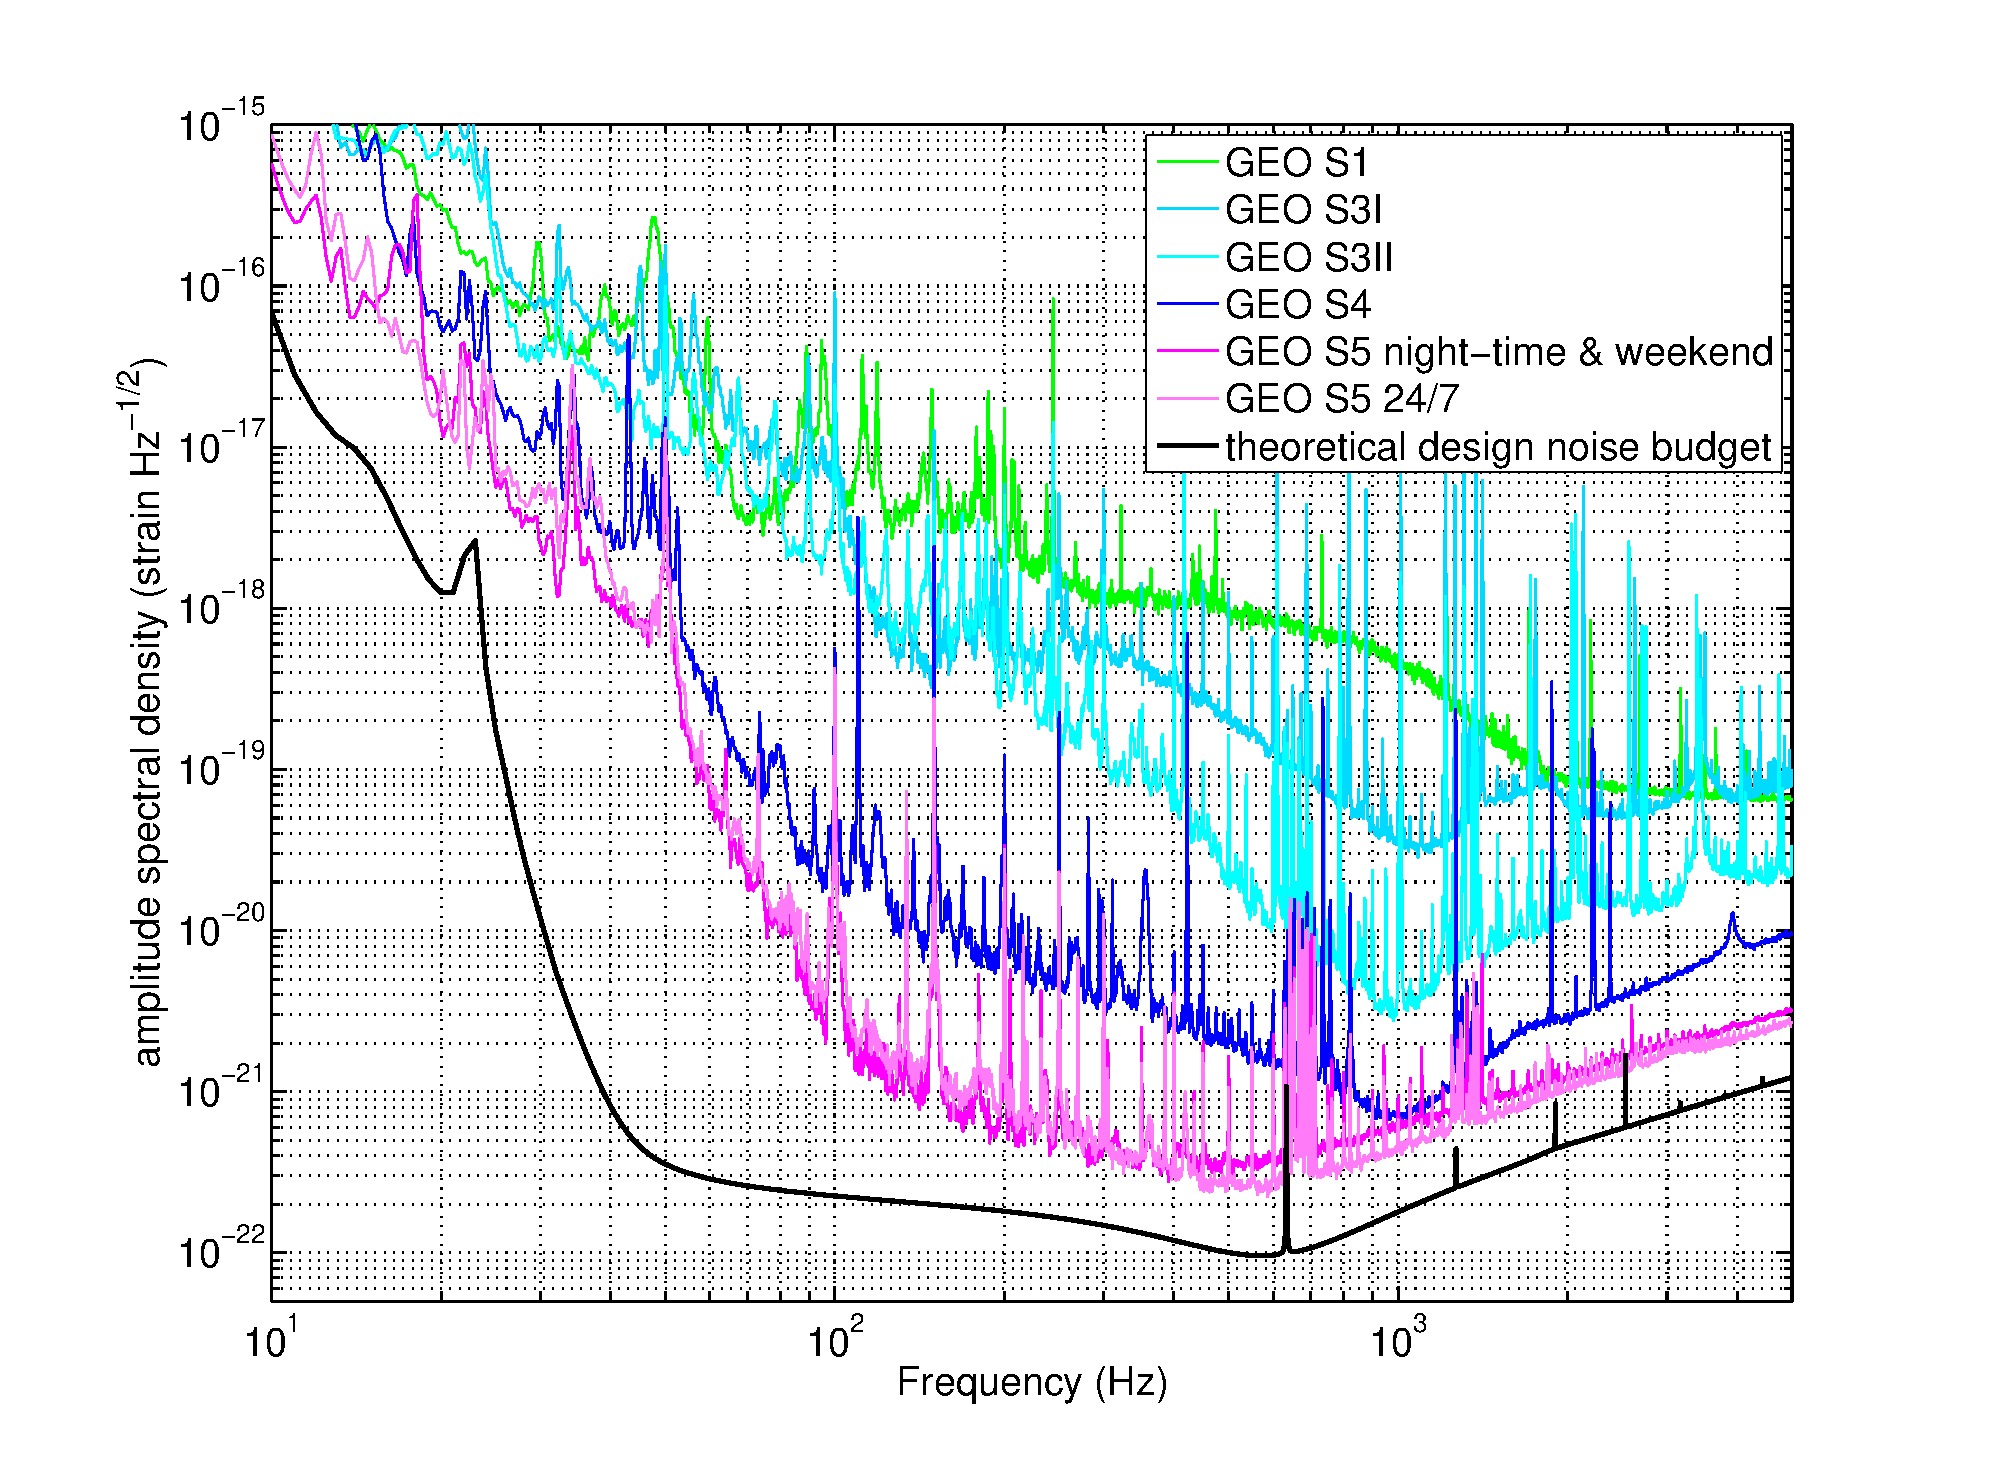
\includegraphics[scale=0.45]{figures/GEOSrunASDs/GEOSrunASDs}}
  \caption[]{The typical strain sensitivities from the GEO600 science runs S1
through S5~\cite{GEOcurves}. Also shown is the theoretical noise budget for the
detector when tuned to 550~Hz -- the operating position for the S5 run.}
\end{figure}}


Following S1 the signal recycling mirror was installed and in late 2003 the
first lock of the fully dual-recycled system was achieved
(see~\cite{Smith:2004, Willke:2004, Grote:2005} for information on the
commissioning of GEO600 as a dual-recycled detector). Other upgrades included the
installation of the final mirrors, suspended as triple pendulums, and with
monolithic final stages. Once installed it was found that there was a radius of
curvature mismatch with one of the mirrors, which had to be compensated for by
carefully heating the mirror. Due to this commissioning effort GEO600 did not
participate in the S2 run. Very soon after the implementation of dual-recycling
GEO600 took part in the S3 run. This occurred over two time intervals from
5\,--\,11 November 2003, dubbed S3I, and from 30 December 2003 to 13 January 2004,
dubbed S3II. During S3I GEO600 operated with the signal-recycling cavity tuned
to $\sim$~1.3~kHz, and had a $\sim$~95\% duty factor, but was then taken
off-line for more commissioning work. In the period between S3I and II various
sources of noise and lock loss were diagnosed and mitigated, including noise
from a servo in the signal recycling cavity and electronic noise on a
photo-diode~\cite{Smith:2004}. This lead to improved sensitivity by up to an
order of magnitude at some frequencies (see Figure~\ref{figure:GEOstrains}). For
S3II the signal recycling cavity was tuned to 1~kHz and, due to the upgrades,
had an increased duty factor of $\sim$~99\%. GEO600 operated during the whole of
S4 (22 February to 24 March 2004), in coincidence with LIGO, with a $\sim$~97\%
duty factor. It used the same optical configuration as S3, but had sensitivity
improvements from a few times to up to an order of magnitude over the S3
values~\cite{Hild:2006a}.


The main changes to the detector after S4 were to shift the resonance condition
of the signal recycling cavity to a lower frequency, 350~Hz, allowing better
sensitivity in the few hundred Hz regime, and increasing the circulating laser
power, with an input power of 10~W. The pre-S5 peak sensitivity was
$\sim$~4~\texttimes~10\super{-22}~\Hz at around 400~Hz, with an inspiral
range of 0.6\,Mpc~\cite{Hild:2006b}. GEO600 did not join S5 at the start of the
LIGO run, but from 21 January 2006 was in a night-and-weekend data-taking mode
whilst noise hunting studies and commissioning were conducted. For S5 the signal
recycling cavity was re-tuned up to 550~Hz. It went into full-time data taking
from 1 May to 16 October 2006, with an instrumental duty factor of 94\%. The
average peak sensitivity during S5 was better than
3~\texttimes~10\super{-22}~\Hz (see~\cite{Willke:2007} for a
summary of GEO600 during S5). After this it was deemed more valuable
for GEO600 to continue more noise hunting and commissioning work, to
give as good a sensitivity as possible for when the LIGO detectors
went offline for upgrading. However, it did continue operating in night-and-weekend mode.


GEO600 continued operating in Astrowatch mode between November 2007 and July
2009 after which upgrades began. The plans for the GEO600 detector are to
continue to use it as a test-bed for more novel interferometric techniques
whilst focusing on increasing in sensitivity at higher frequencies (greater than
a few hundred Hz). This project is called GEO-HF~\cite{Willke:2006}. The
upgrading towards GEO-HF has been taking place since Summer
2009~\cite{Grote:2010}. The main upgrades started during 2009 were to
change the read-out scheme from an RF read-out to a DC read-out system~\cite{Hild:2009}
(also see Section~\ref{sec:readout}), install an output mode cleaner, place the
read-out system in vacuum, injecting squeezed light~\cite{Vahlbruch:2008,
Chelkowski:2007} into the output port, and finally increasing the input laser
power to 35~W. Running the interferometer with squeezed light will be the first
demonstration of a full-scale gravitational-wave detector operating beyond the
standard quantum limit. GEO-HF participated in S6 in an overnight and weekend
mode, alongside a commissioning schedule, and is continuing in this mode
following the end of S6.


\subsubsection{Virgo}


In summer 2002 Virgo completed the commissioning of the central area
interferometer, consisting of a power-recycled Michelson interferometer, but
without the 3~km Fabry--P\'{e}rot arm cavities. Over the next couple of years
various steps were made towards commissioning the full-size interferometer. In
early 2004 first lock with the 3~km arms was achieved, but without
power-recycling, and by the end of 2004 lock with power recycling was achieved.
During summer 2005 the commissioning runs provided order-of-magnitude
sensitivity improvements, with a peak sensitivity of
6~\texttimes~10\super{-22}~\Hz at 300~Hz, and an inspiral range
of over 1~Mpc. In late 2005 several major upgrades brought Virgo to
its final configuration. See~\cite{Acernese:2004, Acernese:2005,
Acernese:2006, Acernese:2007} for more detailed information on the
commissioning of the detector.


Virgo joined coincident observations with the LIGO and GEO600 S5 run with 10
weekend science runs (WSRs) starting in late 2006 until March 2007. Over this
time improvements were made mainly in the mid-to-low frequency regime
($\lesssim$~300~Hz). Full-time data taking, under the title of Virgo
Science run 1 (VSR1), began on 18 May 2007 and ended with the end of
S5 on 1 October 2007. During VSR1, the science-mode duty factor was
81\% and by the end of the run maximum neutron-star--binary inspiral
range was frequently up to about 4.5~Mpc. The best sensitivity curves
for WSR1, WSR10 and VSR1 can be seen in Figure~\ref{figure:Virgostrains}.


At the same time as commissioning for Enhanced LIGO was taking place there was
also a similar effort to upgrade the Virgo detector, called Virgo+. The main
upgrade was to the lasers to increase their power from 10 to 25~W at the input
mode cleaner, with upgrades also to the thermal compensation system on the
mirrors, the control electronics, mode cleaners and injection optics
\cite{Acernese:2008b, AdvVirgoWhitepaper}. Virgo+ started taking data
with Enhanced LIGO for Virgo Science Run 2 (VSR2) and sensitivities of
Virgo+ close to the initial Virgo design sensitivity were
reached. VSR2 finished on 8 January 2010 to allow for further
commissioning and noise hunting. This was followed by VSR3, which
began on 11 August 2010 and ran until 20 October 2010. Further Virgo+
runs are expected during 2011. Following these the upgrades to
Advanced Virgo will begin.


% Virgo typical strain sensitivities
\epubtkImage{figures/VirgoSrunASDs/VirgoSrunASDs.png}{%
\begin{figure}[htbp]
  \centerline{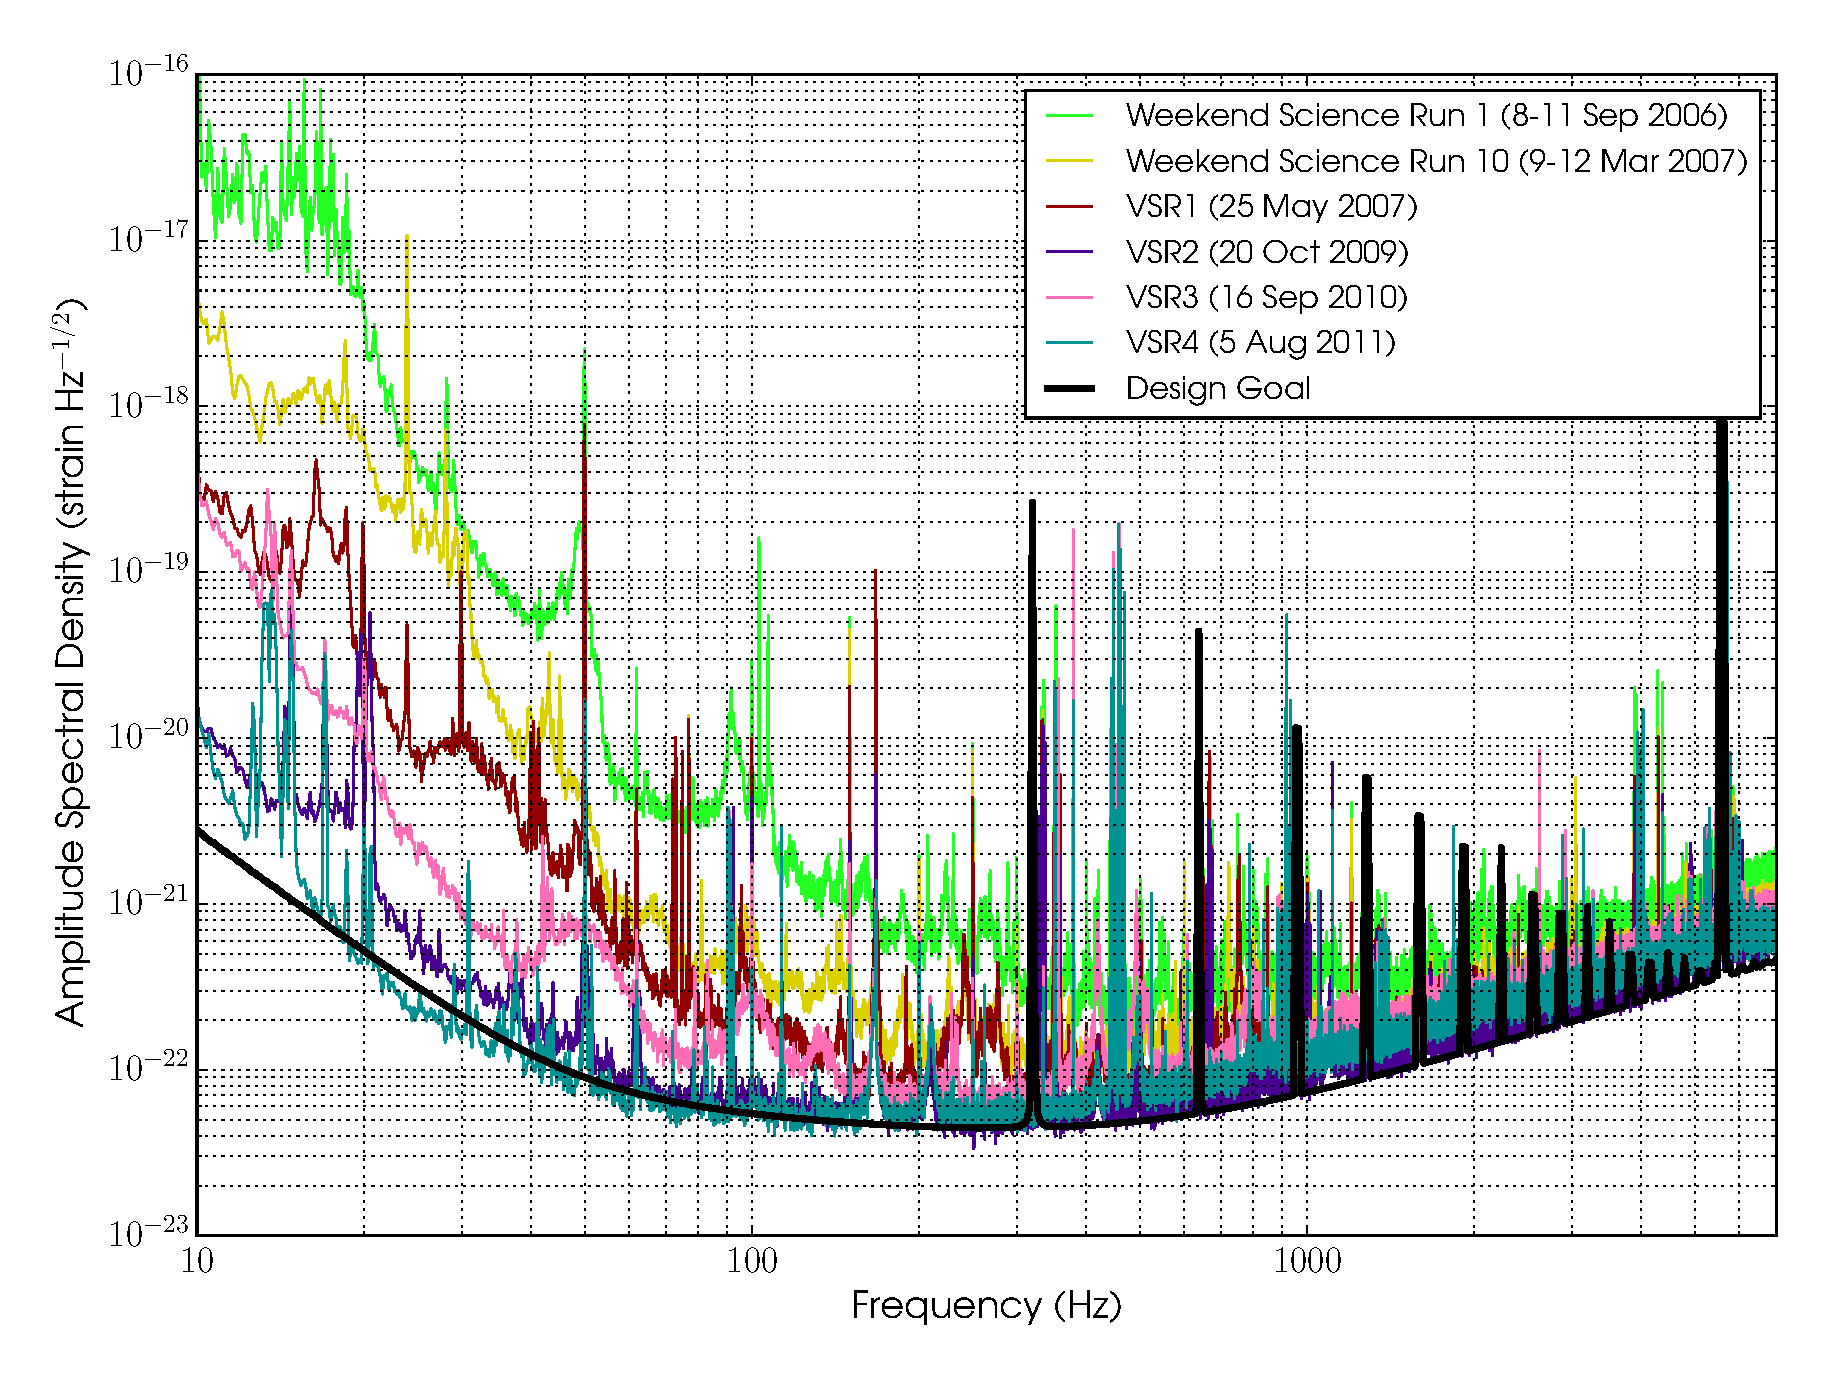
\includegraphics[scale=0.45]{figures/VirgoSrunASDs/VirgoSrunASDs}}
  \caption[]{\label{figure:Virgostrains}
The best strain sensitivities from the Virgo weekend and full
time science runs WSR1, WSR10, VSR1 and VSR2~\cite{VIRGOcurves, VSR2paper}.
}
\end{figure}}


\input{Section6_7}

% second generation detector design strain sensitivities
\epubtkImage{figures/advcurves/advcurves.png}{%
\begin{figure}[htbp]
  \centerline{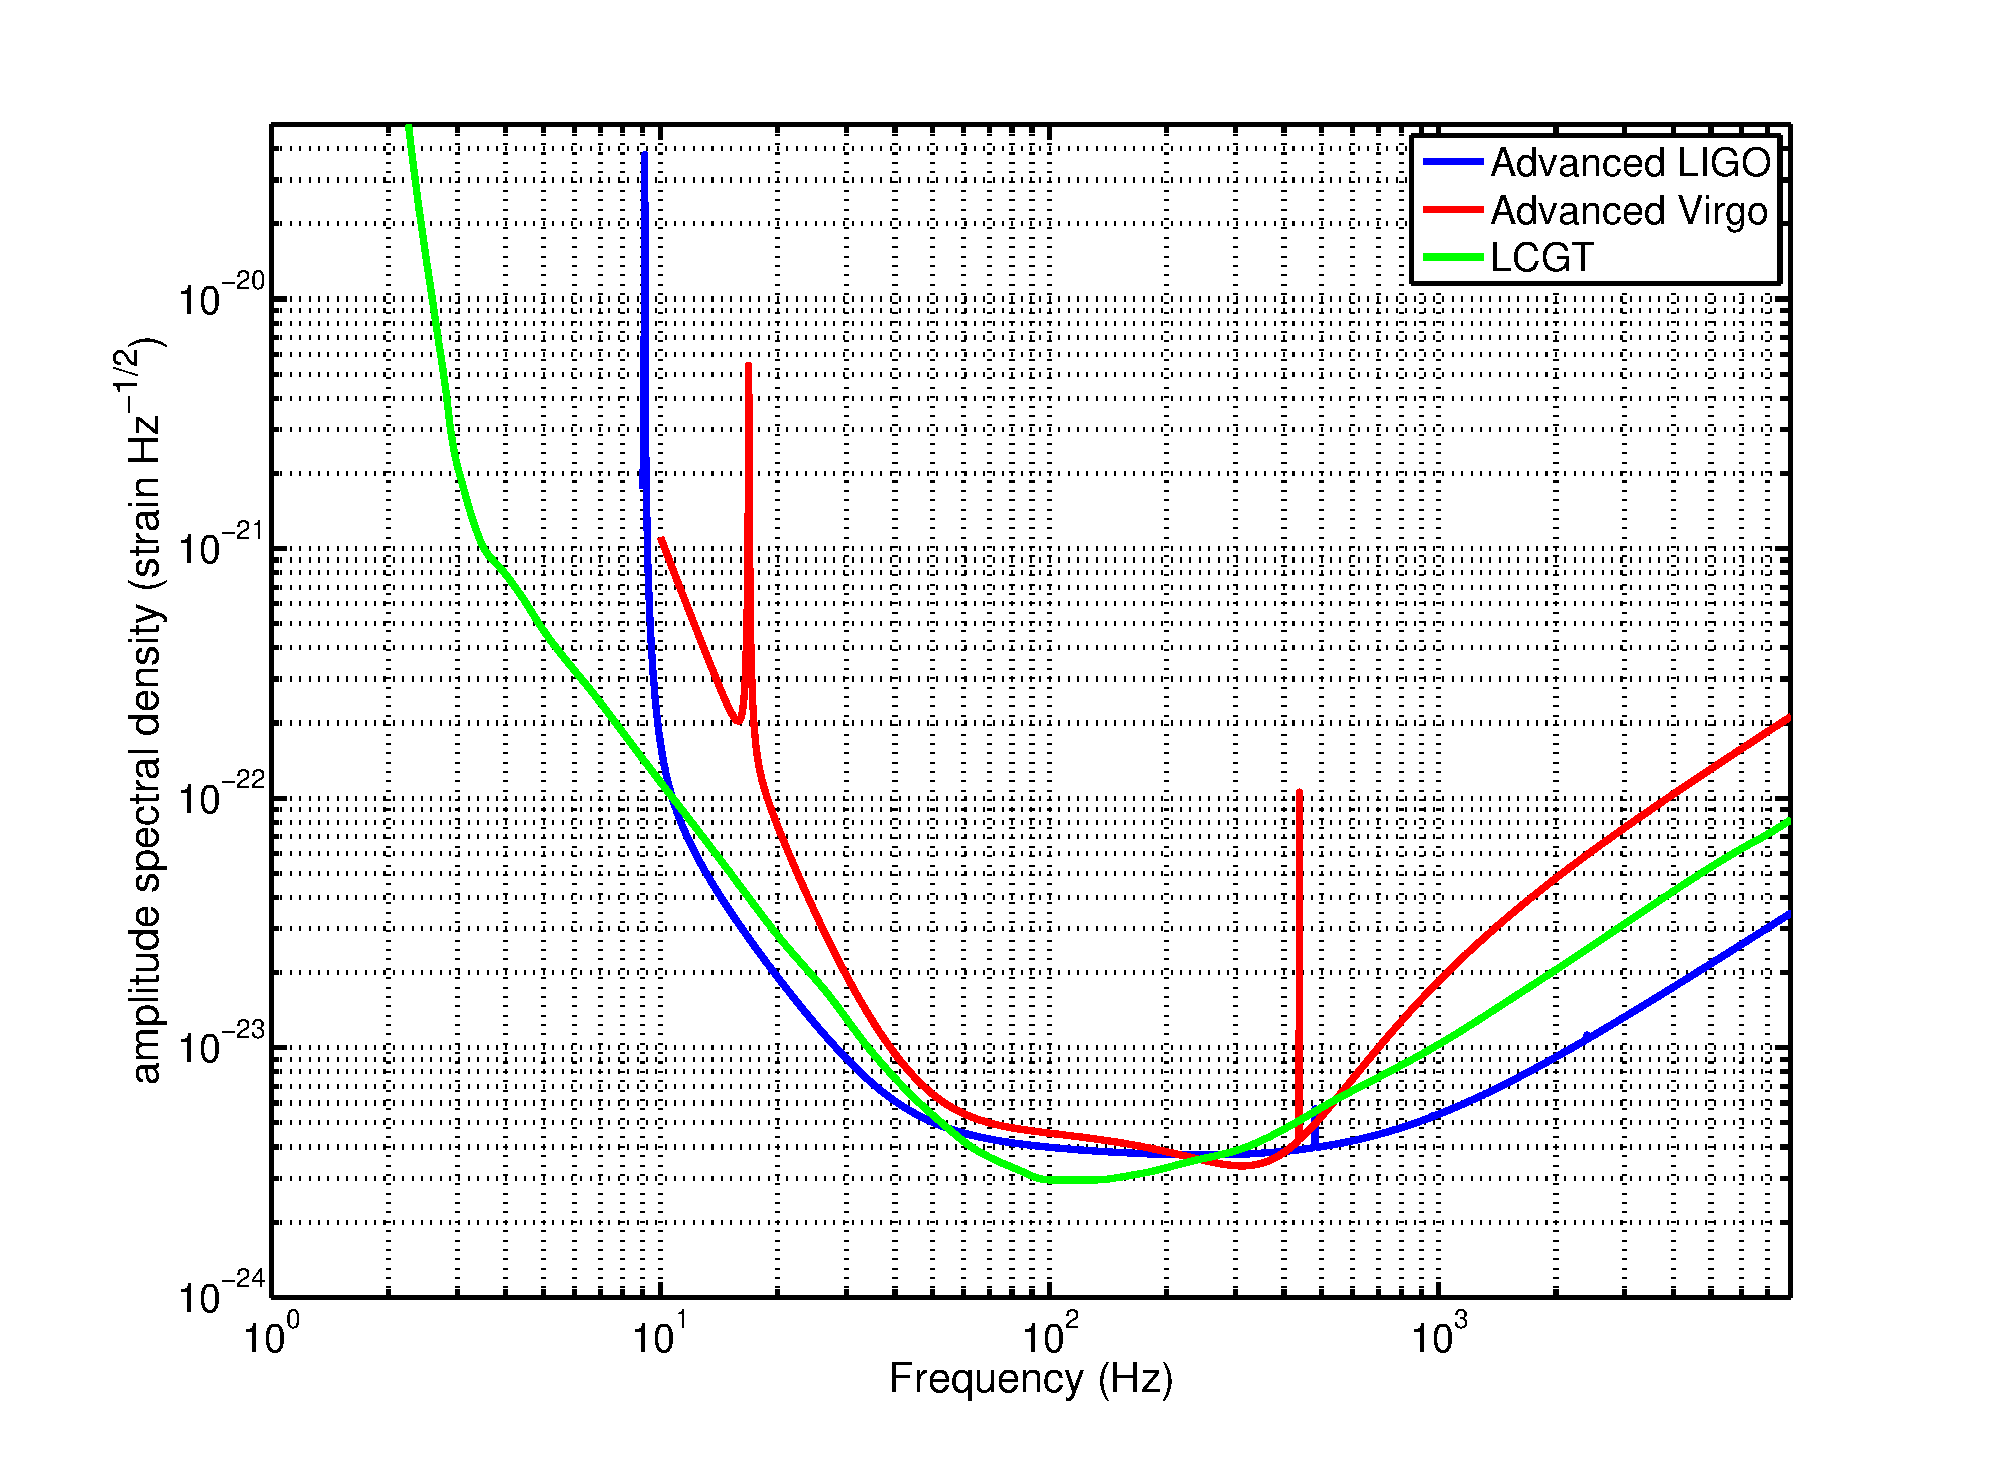
\includegraphics[scale=0.4]{figures/advcurves/advcurves}}
  \caption[]{Design sensitivity curves for the Advanced LIGO, Advanced Virgo
and LCGT second-generation detectors. The Advanced LIGO curve comes from
\cite{Harry:2010}, the Advanced Virgo curve comes
from~\cite{AdvVirgoweb}, and the LCGT curve comes
from~\cite{Arai:2009}. These curves are based on specific
configurations of the detectors and are therefore subject to change.}
\end{figure}}

\input{Section6_8}

\epubtkImage{figures/etcurve/etcurve.png}{%
\begin{figure}[htbp]
  \centerline{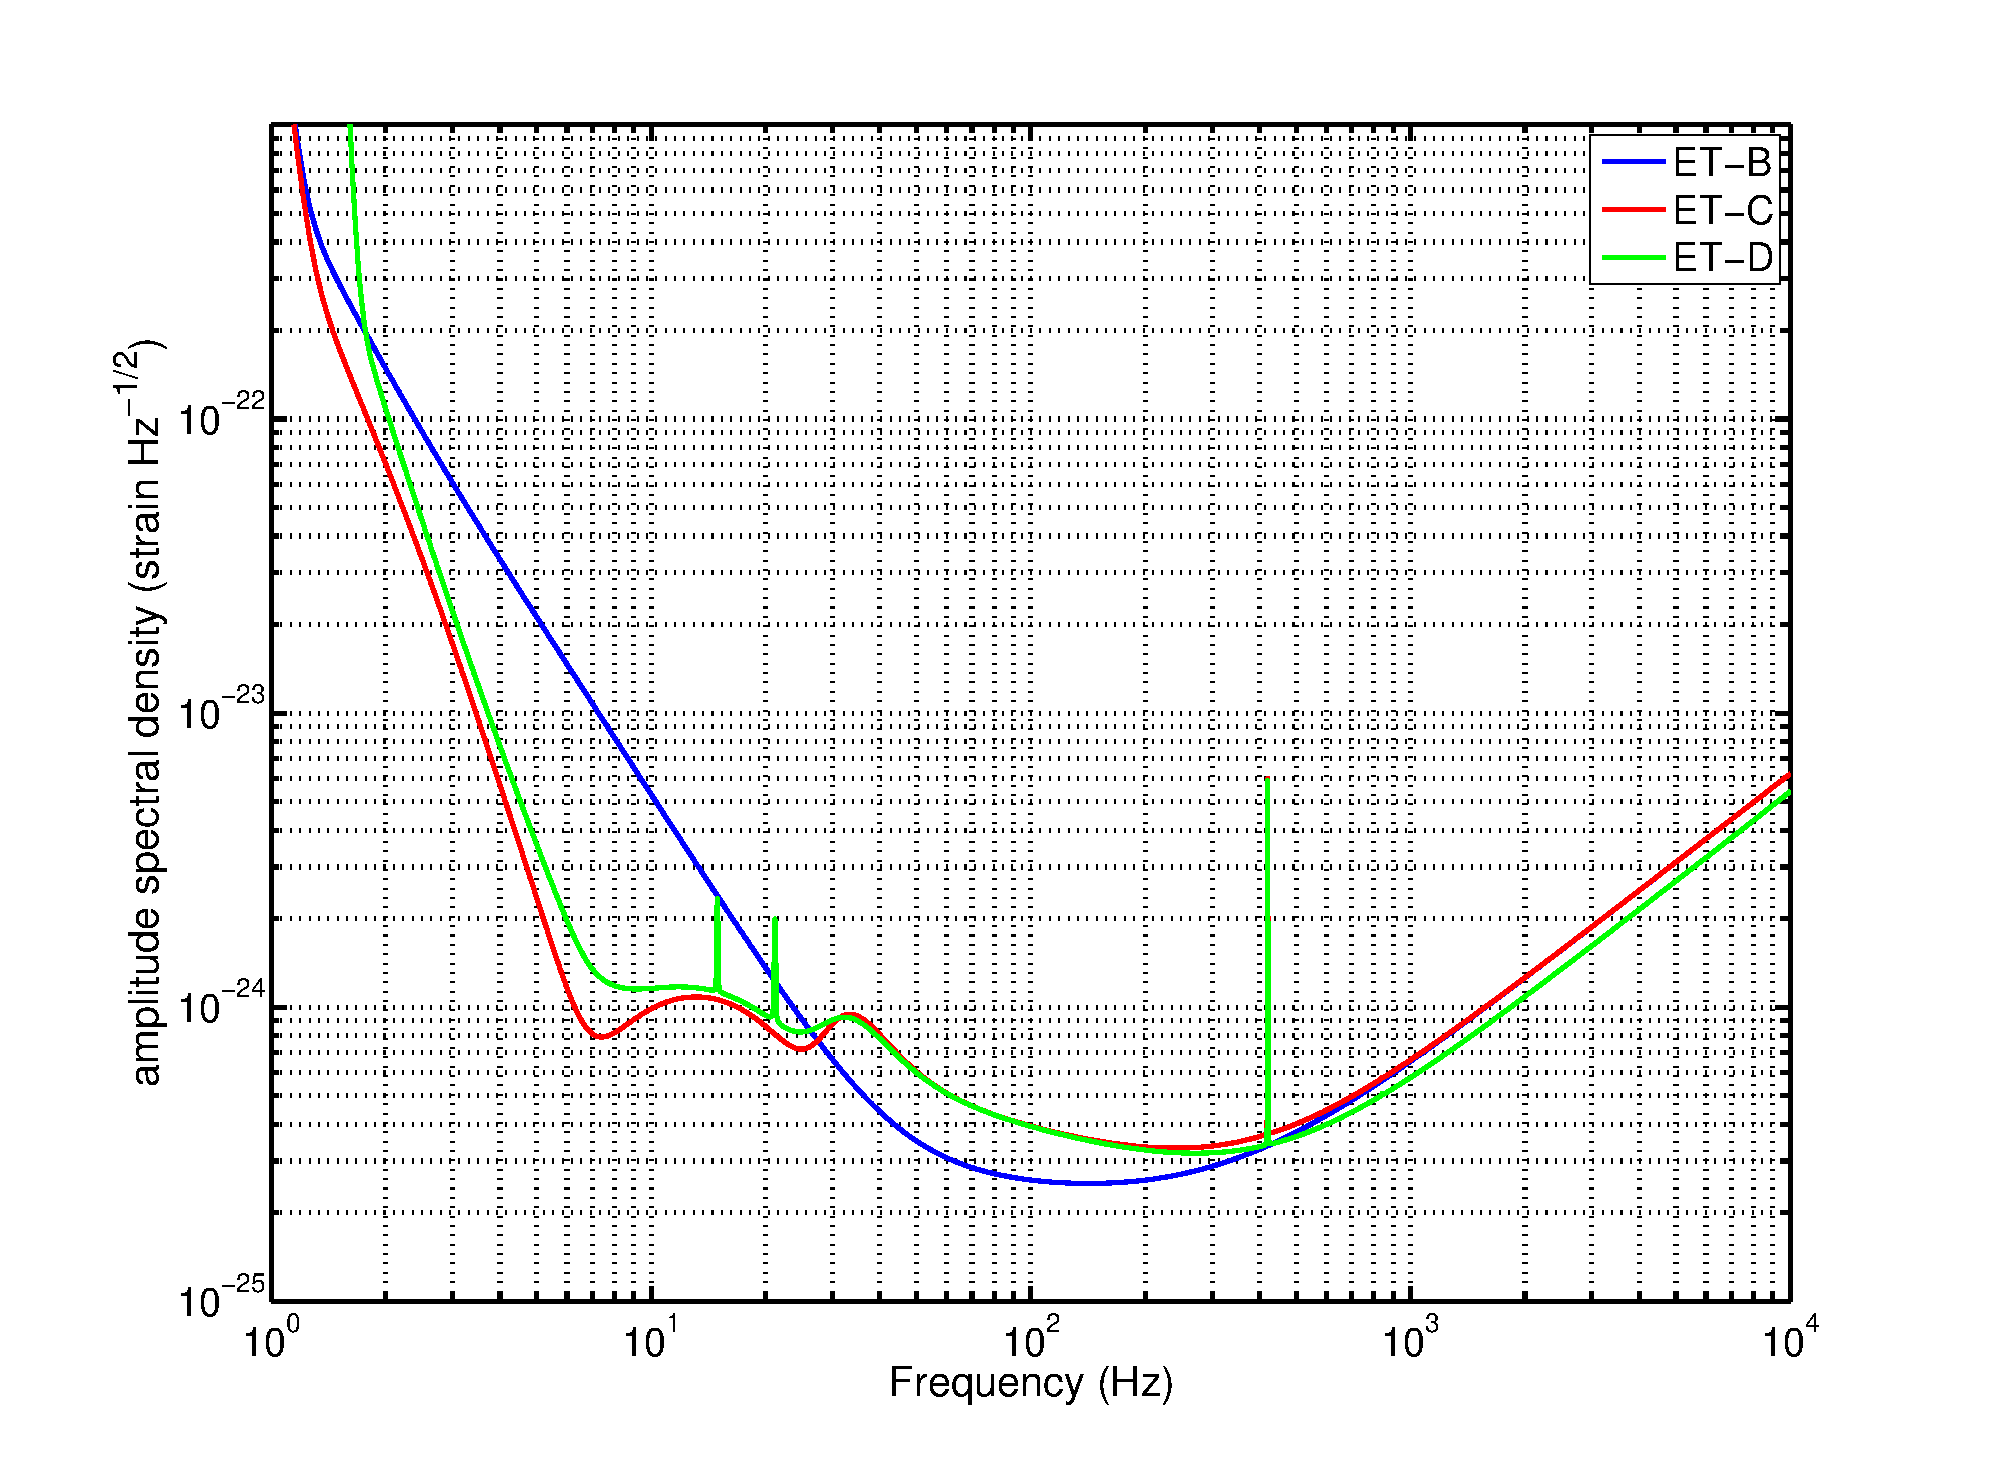
\includegraphics[scale=0.4]{figures/etcurve/etcurve}}
  \caption[]{\label{fig:etsens}
Potential sensitivities of the Einstein Telescope for 3 different
design concepts (ET-B~\cite{Hild:2008}, ET-C~\cite{Hild:2010b} and ET-D
\cite{Hild:2010}, where the curves are available from~\cite{etcurves}) and the
Cosmic Explorer telescope~\cite{2016arXiv160708697A}.}
\end{figure}}

%%%%%%%%%%%%%%%%%%%%%%%%%%%%%%%%%%%%%%%%%%%%%%%%%%%%%%%%%%%%%%%%%%%%%%%%%%%%%%%%
%%%%%%%%%%%%%%%%%%%%%%%%%%%%%%%%%%%%%%%%%%%%%%%%%%%%%%%%%%%%%%%%%%%%%%%%%%%%%%%%
%%%%%%%%%%%%%%%%%%%%%%%%%%%%%%%%%%%%%%%%%%%%%%%%%%%%%%%%%%%%%%%%%%%%%%%%%%%%%%%%

\newpage

\input{Section7_1}

\epubtkImage{figures/lisacurve/lisacurve.png}{%
\begin{figure}[htbp]
  \centerline{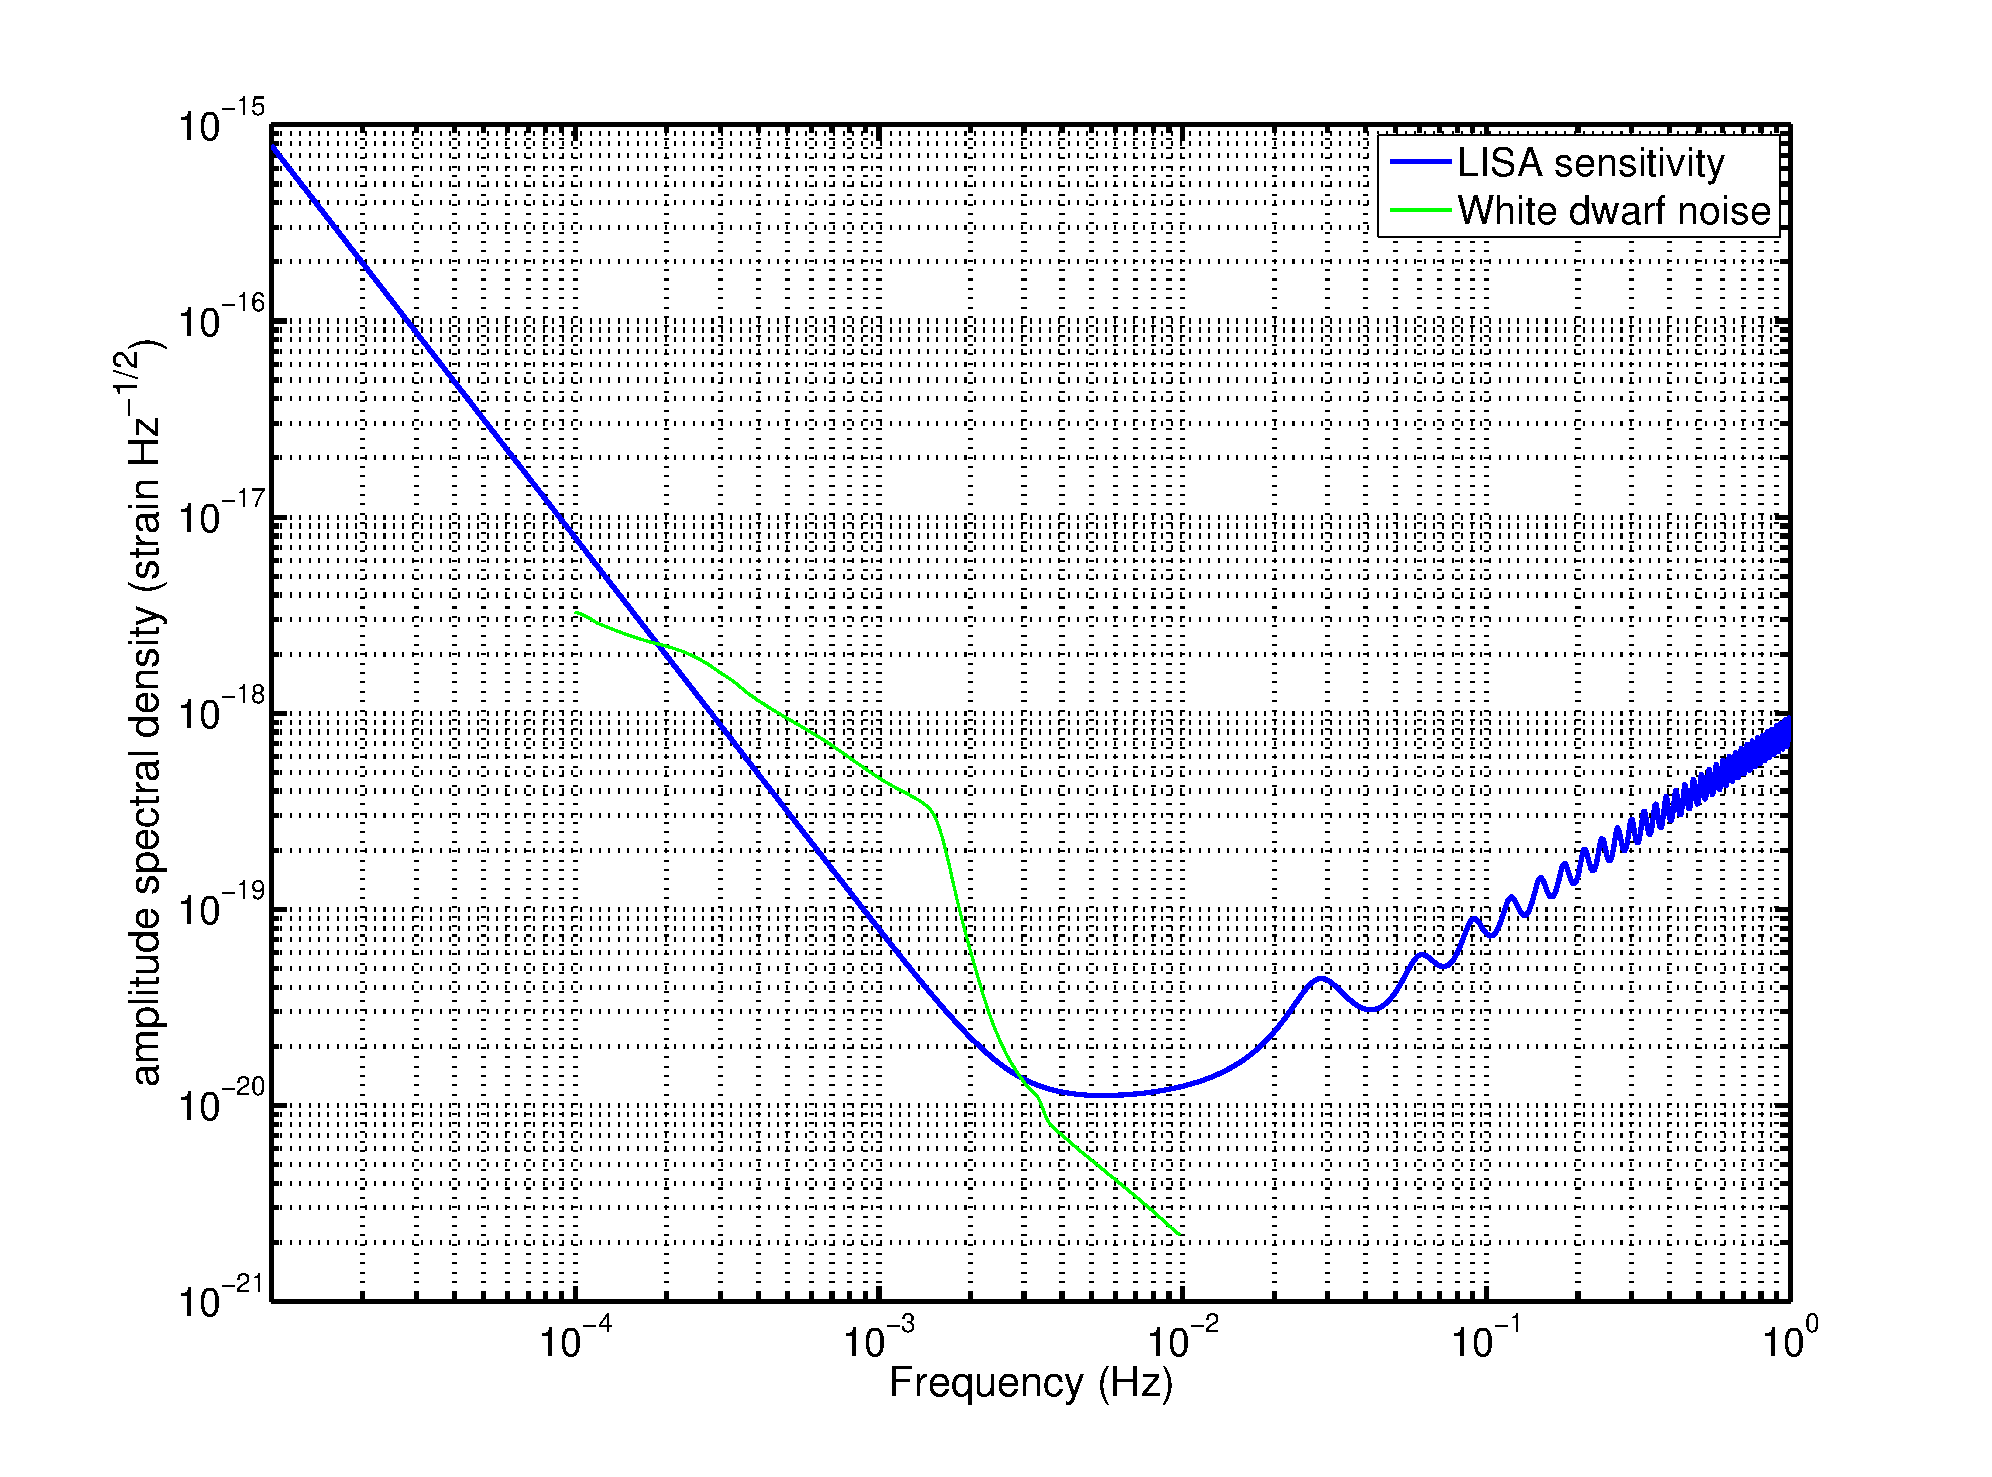
\includegraphics[scale=0.4]{figures/lisacurve/lisacurve}}
  \caption[]{A design sensitivity amplitude spectral density curve for LISA
created using the standard parameters in the online generator
at~\cite{lisasens}. The curve assumes equal length arms, sensitivity
averaged over the whole sky and all polarisations, and an SNR of
1. Also included is a curve showing the expected background noise from
galactic white-dwarf--binary systems, which will dominate over the
instrumental noise in the range from $\approx$~0.1\,--\,1~mHz.}
\end{figure}}

\input{Section7_2}

\epubtkImage{figures/fig8/fig8.png}{%
\begin{figure}[htbp]
  \centerline{\includegraphics[scale=0.4]{figures/fig8/fig8}}
  \caption[]{\label{figure:LISA}
The proposed LISA detector.}
\end{figure}}

\input{Section7_3}


%%%%%%%%%%%%%%%%%%%%%%%%%%%%%%%%%%%%%%%%%%%%%%%%%%%%%%%%%%%%%%%%%%%%%%%%%%%%%%%%
%%%%%%%%%%%%%%%%%%%%%%%%%%%%%%%%%%%%%%%%%%%%%%%%%%%%%%%%%%%%%%%%%%%%%%%%%%%%%%%%
%%%%%%%%%%%%%%%%%%%%%%%%%%%%%%%%%%%%%%%%%%%%%%%%%%%%%%%%%%%%%%%%%%%%%%%%%%%%%%%%

%\newpage

\input{Section8.tex}

%%%%%%%%%%%%%%%%%%%%%%%%%%%%%%%%%%%%%%%%%%%%%%%%%%%%%%%%%%%%%%%%%%%%%%%%%%%%%%%%
%%%%%%%%%%%%%%%%%%%%%%%%%%%%%%%%%%%%%%%%%%%%%%%%%%%%%%%%%%%%%%%%%%%%%%%%%%%%%%%%
%%%%%%%%%%%%%%%%%%%%%%%%%%%%%%%%%%%%%%%%%%%%%%%%%%%%%%%%%%%%%%%%%%%%%%%%%%%%%%%%

\bigskip

%\newpage

\section{Acknowledgements}
\label{section:acknowledgements} 

We are grateful to the LSC and the Virgo groups for the use of some of their
figures. We are indebted to STFC (U.K.), NSF (U.S.A.), the University of
Glasgow, the Royal Society of Edinburgh, and the Royal Society for support.



%%%%%%%%%%%%%%%%%%%%%%%%%%%%%%%%%%%%%%%%%%%%%%%%%%%%%%%%%%%%%%%%%%%%%%%%%%%%%%%%%%%
%%%%%%%%%%%%%%%%%%%%%%%%%%%%%%%%%%%%%%%%%%%%%%%%%%%%%%%%%%%%%%%%%%%%%%%%%%%%%%%%%%%
%%%%%%%%%%%%%%%%%%%%%%%%%%%%%%%%%%%%%%%%%%%%%%%%%%%%%%%%%%%%%%%%%%%%%%%%%%%%%%%%%%%

\newpage

\bibliography{bibliography/biblio}

\end{document}
